\section{Selecting Parameters for High-Level Synthesis for FPGAs}
\label{sec:FPGA}

FPGAs are reprogrammable circuits that enable writing specialized hardware
specifications for a variety of applications using the same chip.
High-Performance Computing tasks that require low power and latency
increasingly switch to FPGAs from GPUs. Hardware specifications are written
using low-level languages such as Verilog and VHDL, making a challenge for
software engineers to leverage FPGA capabilities.  This became increasingly
relevant by the adaptation of FPGAs for data
centers~\cite{caulfield2016cloud}\footnote{\url{https://cloud.baidu.com/product/fpga.html}
[Accessed in 28/07/2017], \\ and
\url{https://aws.amazon.com/ec2/instance-types/f1/} [Accessed in 28/07/2017]},
a field dominated by software engineers.

Essential support for software engineers can be provided by High-Level
Synthesis (HLS), the process of generating hardware descriptions from
high-level code.  HLS lowers the complexity of hardware design from the point
of view of software engineering and has become increasingly viable as part of
the FPGA design methodology, with support from vendor HLS
tools~\cite{singh2011implementing, feist2012vivado} for C/C++ and OpenCL. The
benefits of higher-level abstractions come with the cost of decreased
application performance, making FPGAs less viable as accelerators.  Thus,
optimizing HLS still requires domain expertise and exhaustive or manual
exploration of design spaces and configurations.

High-Level Synthesis is an \NP{}-Complete problem~\cite{canis2015legup} and a
common strategy for its solution involves the divide-and-conquer
approach~\cite{coussy2009introduction}.  The most important sub-problems to
solve are \textit{scheduling}, where operations are assigned to specific clock
cycles, and \textit{binding}, where operations are assigned to specific
hardware functional units, which can be shared between operations.
LegUp~\cite{canis2013legup} is an open-source HLS tool implemented as a
compiler pass for the LLVM Compiler Infrastructure~\cite{chris2004llvm}.  It
receives code in LLVM's intermediate representation as input and produces as
output a hardware description in Verilog.  LegUp exposes configuration
parameters of its HLS process, set with a configuration file.

This section presents an autotuner for LegUp HLS parameters implemented using
the OpenTuner framework.  The autotuner targeted 8 hardware metrics obtained
from
Quartus~\footnote{\url{https://www.altera.com/products/design-software/fpga-design/quartus-prime/overview.html}
[Accessed in 18/07/2017]}, for applications of the CHStone HLS benchmark
suite~\cite{hara2008chstone} in the Intel StratixV FPGA.  The program to be
configured here is LegUp and the search space is composed of approximately
$10^{126}$ possible combinations of HLS parameters.  Such a large search space
is unfeasible to search exhaustively or by hand.

One of the obstacles we faced was making accurate predictions for hardware
metrics from a set of HLS parameters. We decided to run our autotuner with the
metrics reported by the lengthier process of hardware synthesis instead.  Our
autotuner's virtualized implementation enables deployment in distributed
environments.  We present data showing that our autotuner found optimized HLS
parameters for CHStone applications that decreased the \textit{Weighted
Normalized Sum} (\textbf{WNS}) of hardware metrics by up to $21.5\%$ on
average, and $10\%$ on average.

\subsection{Large Measurement Time}
\label{sec:bigtime}

The defining characteristic of this autotuning experiment is the potentially
large time it takes to synthesize hardware from specifications in hardware
description languages, which takes from minutes to hours. The process of
generating those specifications from high-level C code is much faster in
comparison, taking only seconds. In contrast to the previous section, the
applications used in this autotuning experiment had a \textit{large measurement
time}. Section~\ref{sec:FPGAautotuner} describes in more detail the High-Level
Synthesis process.

\begin{figure}[htpb]
    \centering
    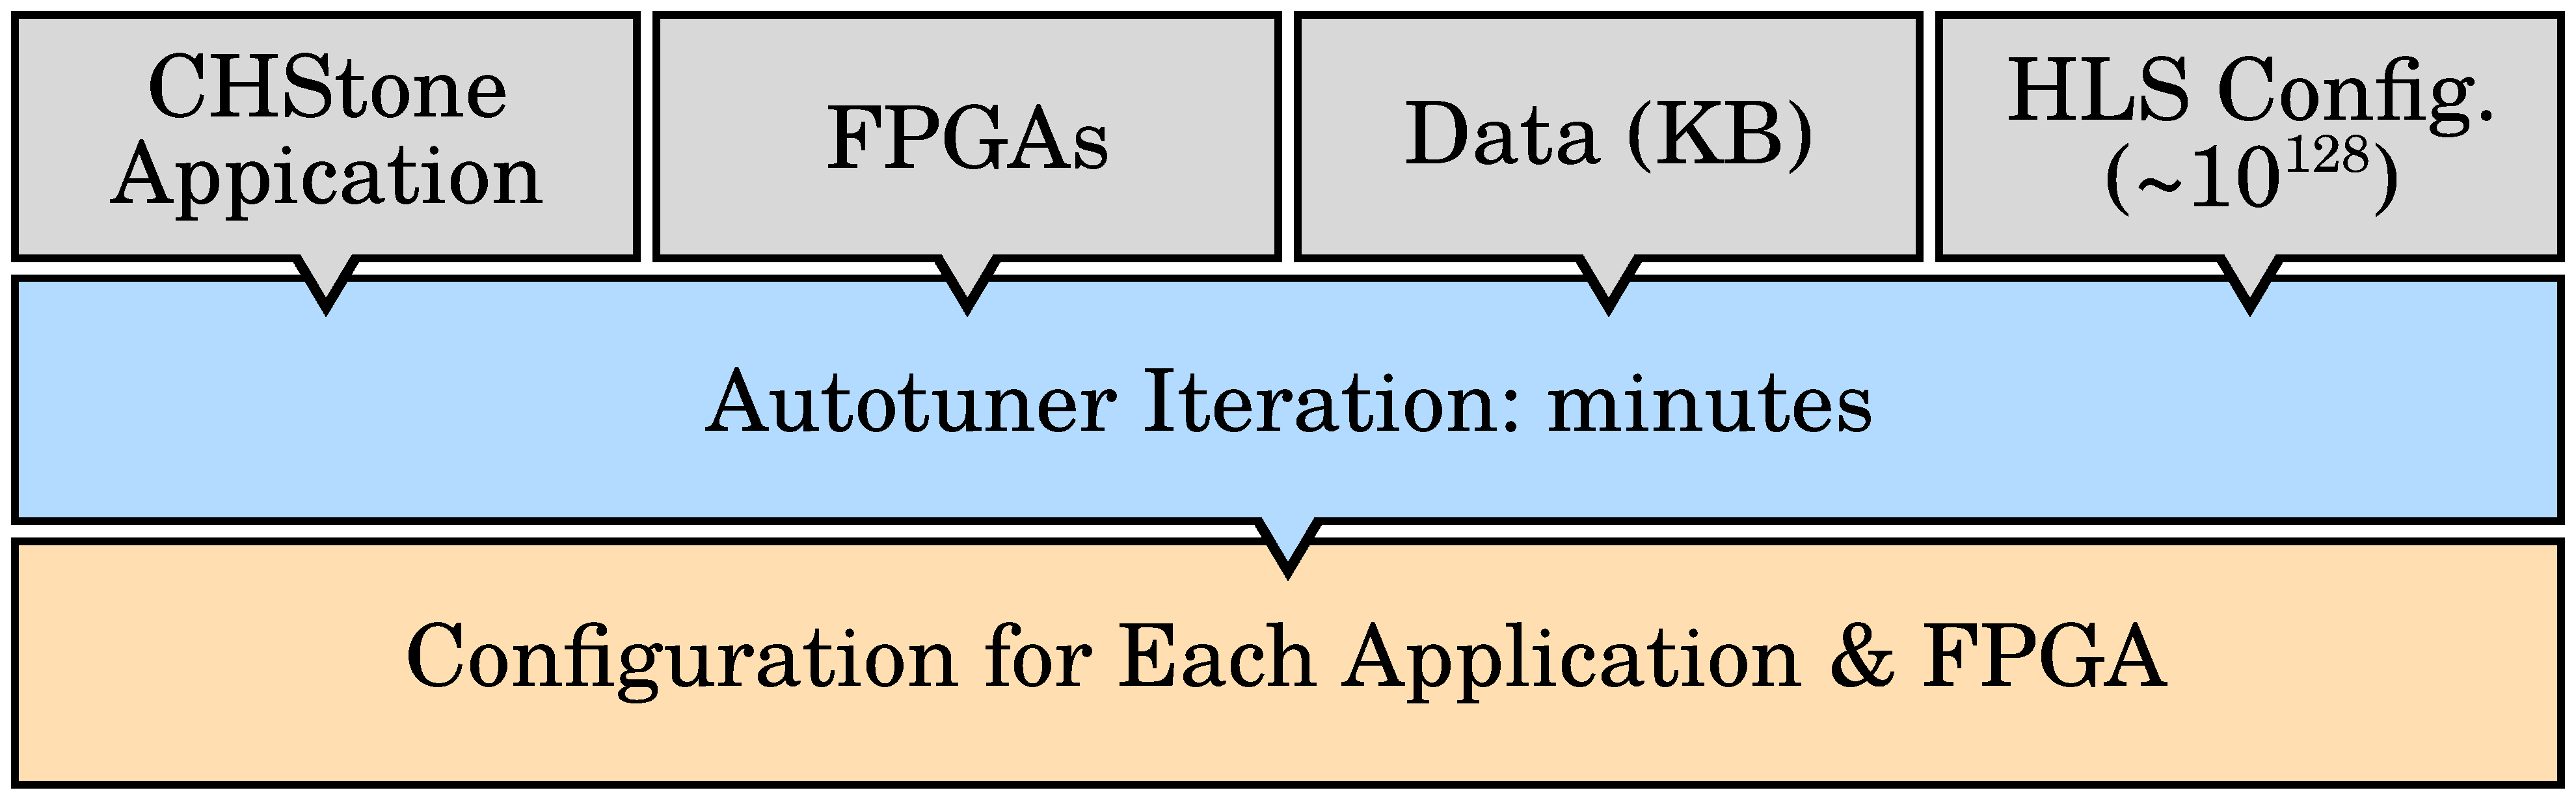
\includegraphics[width=.65\textwidth]{./images/overview_fpgas_small}
    \caption{Autotuner representation and time scale of our experiments}
    \label{fig:overview-fpgas-small}
\end{figure}

Figure~\ref{fig:overview-fpgas-small} shows a representation of our autotuner
for this experiment, and illustrates its time scale.  The autotuner,
represented by the light blue box, receives as input a CHStone application, a
target FPGA, input data for the application in the order of Kilobytes and a
search space composed of LegUp's HLS parameters. The autotuner outputs an HLS
configuration for each application and FPGA.

\begin{figure}[htpb]
    \centering
    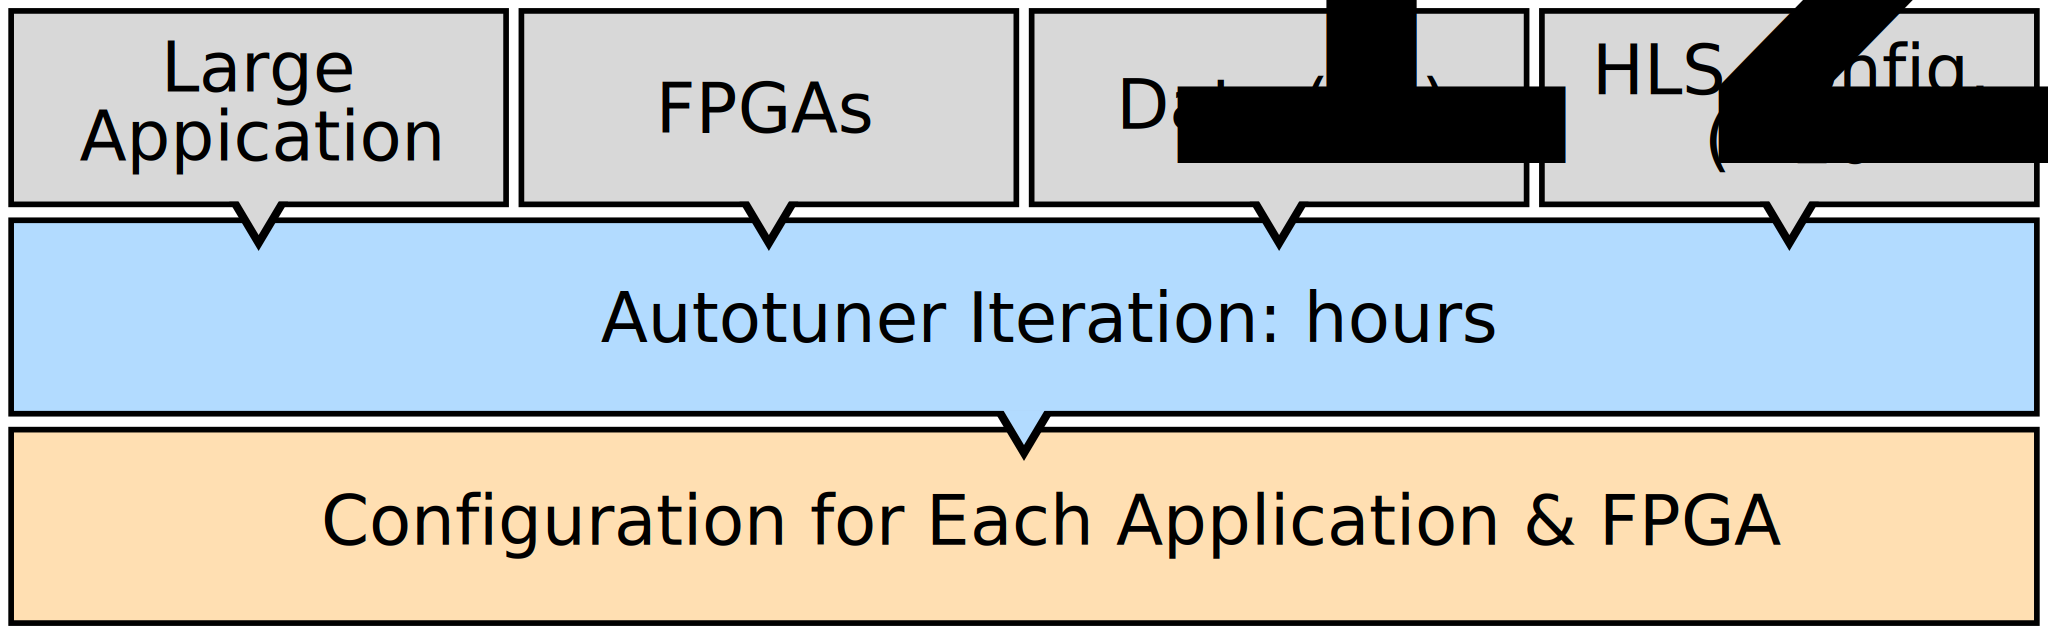
\includegraphics[width=.65\textwidth]{./images/overview_fpgas_big}
    \caption{Autotuner representation and time scale of more complex FPGA
    applications}
    \label{fig:overview-fpgas-big}
\end{figure}

The applications from CHStone, presented further in Table~\ref{tab:chstone},
are very simple benchmark applications, and generating hardware for them takes
time in the order of minutes. Generating hardware for more complex FPGA
applications can take several hours. Figure~\ref{fig:overview-fpgas-big} shows
a representation and time scale for an autotuner that targets complex FPGA
applications. Each iteration now takes several hours, and limits the
configurations that can be tested per hour.

We worked around this limitation in this experiment by implementing a
virtualized autotuner using Docker containers, which enabled parallel
measurements of different configurations. The lack of support in OpenTuner for
a distributed execution of measurements also limited this experiment, since our
already virtualized approach could explore more search space in the same time
if it was deployed in more connected machines.

Applications with large measurement time still present a challenge for our
current autotuning approach, even with a tool that can achieve distributed
execution of measurements, because the quality of the solutions still depend on
the velocity of exploration of the search space.  To mitigate this problem and
enable the autotuning of applications with large measurement times, which can
be thought of as\textit{expensive-to-evaluate functions}, we are going to study
the development of suitable experimental designs. We will work in this
direction in collaboration and supervision of professors Arnaud Legrand, Brice
Videau and Jean-Marc Vincent from the Université de Grenoble Alpes, in
Grenoble, France.

\subsection{Background}
\label{sec:FPGAbackground}

In this section we discuss background work related to HLS tools,
and autotuning for FPGAs.

\paragraph{Tools for HLS}

Research tools for High-Level Synthesis have been developed as well as vendor
tools \cite{singh2011implementing, feist2012vivado}. Villareal \emph{et
al.}~\cite{villarreal2010designing} implemented extensions to the Riverside
Optimizing Compiler for Configurable Circuits (ROCCC), which also uses the LLVM
compiler infrastructure, to add support for generating VHDL from C code.
Implemented within GCC, GAUT~\cite{coussy2010gaut} is an open-source HLS tool
for generating VHDL from C/C++ code. Other HLS tools such as
Mitrion~\cite{kindratenko2007mitrion}, Impulse~\cite{antola2007novel} and
Handel~\cite{loo2002handel} also generate hardware descriptions from C code.
We refer the reader to the survey from Nane \emph{et al.}~\cite{nane2016survey}
for a comprehensive analysis of recent approaches to HLS.

\paragraph{Autotuning for FPGAs}

Recent works study autotuning approaches for FPGA compilation.  Xu et
al.~\cite{xu2017parallel} used distributed OpenTuner instances to optimize the
compilation flow from hardware description to bitstream.  They optimize
configuration parameters from the Verilog-to-Routing (VTR)
toolflow~\cite{luu2014vtr} and target frequency, wall-clock time and logic
utilization.  Huang et al.~\cite{huang2015effect} study the effect of LLVM pass
ordering and application in LegUp's HLS process, demonstrating the complexity
of the search space and the difficulty of its exhaustive exploration.  They
exhaustively explore a subset of LLVM passes and target logic utilization,
execution cycles, frequency, and wall-clock time.  Mametjanov \emph{et
al.}~\cite{mametjanov2015autotuning} propose a machine-learning-based approach
to tune design parameters for performance and power consumption.  Nabi and
Vanderbauwhede~\cite{nabi2016fast} present a model for performance and resource
utilization for designs based on an intermediate representation.

\subsection{Autotuner \& Search Space}
\label{sec:FPGAautotuner}

This section describes our autotuner implementation, the LegUp HLS parameters
selected for tuning, and the autotuning metrics used to measure the quality of
HLS configurations.

\subsubsection{Autotuner}

We implemented our autotuner with OpenTuner~\cite{ansel2014opentuner}, using
ensembles of search techniques to find an optimized selection of
LegUp~\cite{canis2015legup} HLS parameters, according to our cost function, for
11 of the CHStone~\cite{hara2008chstone} applications.

\begin{figure}[htpb]
    \centering
    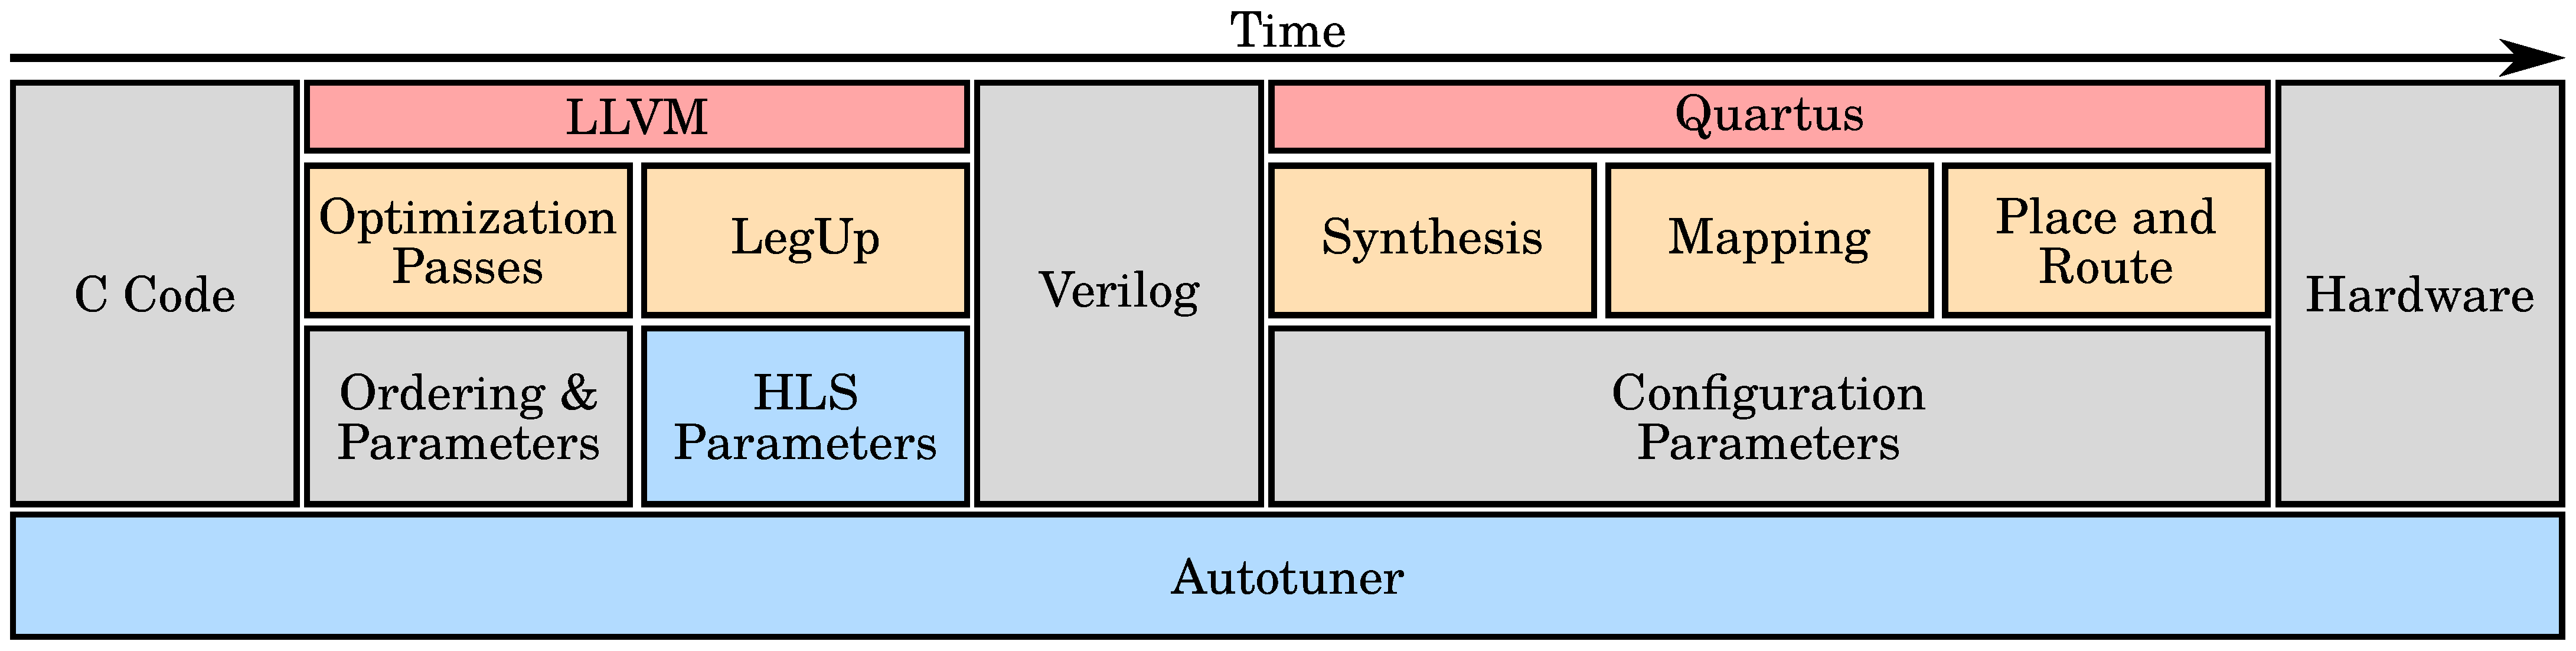
\includegraphics[width=0.8\textwidth]{fpga-stack}
    \caption{High-Level Synthesis compilation process. The autotuner search space at the HLS stage is highlighted in blue}
    \label{fig:fpga-stack}
\end{figure}

Figure \ref{fig:fpga-stack} shows the steps to generate a hardware description
from C code. It also shows the Quartus steps to generate bitstreams from
hardware descriptions and to obtain the hardware metrics we targeted. Our
autotuner used LegUp's HLS parameters as the search space, but it completed the
hardware generation process to obtain metrics from Quartus, as represented by
blue highlights in Figure \ref{fig:fpga-stack}.

\begin{figure}[htpb]
    \centering
    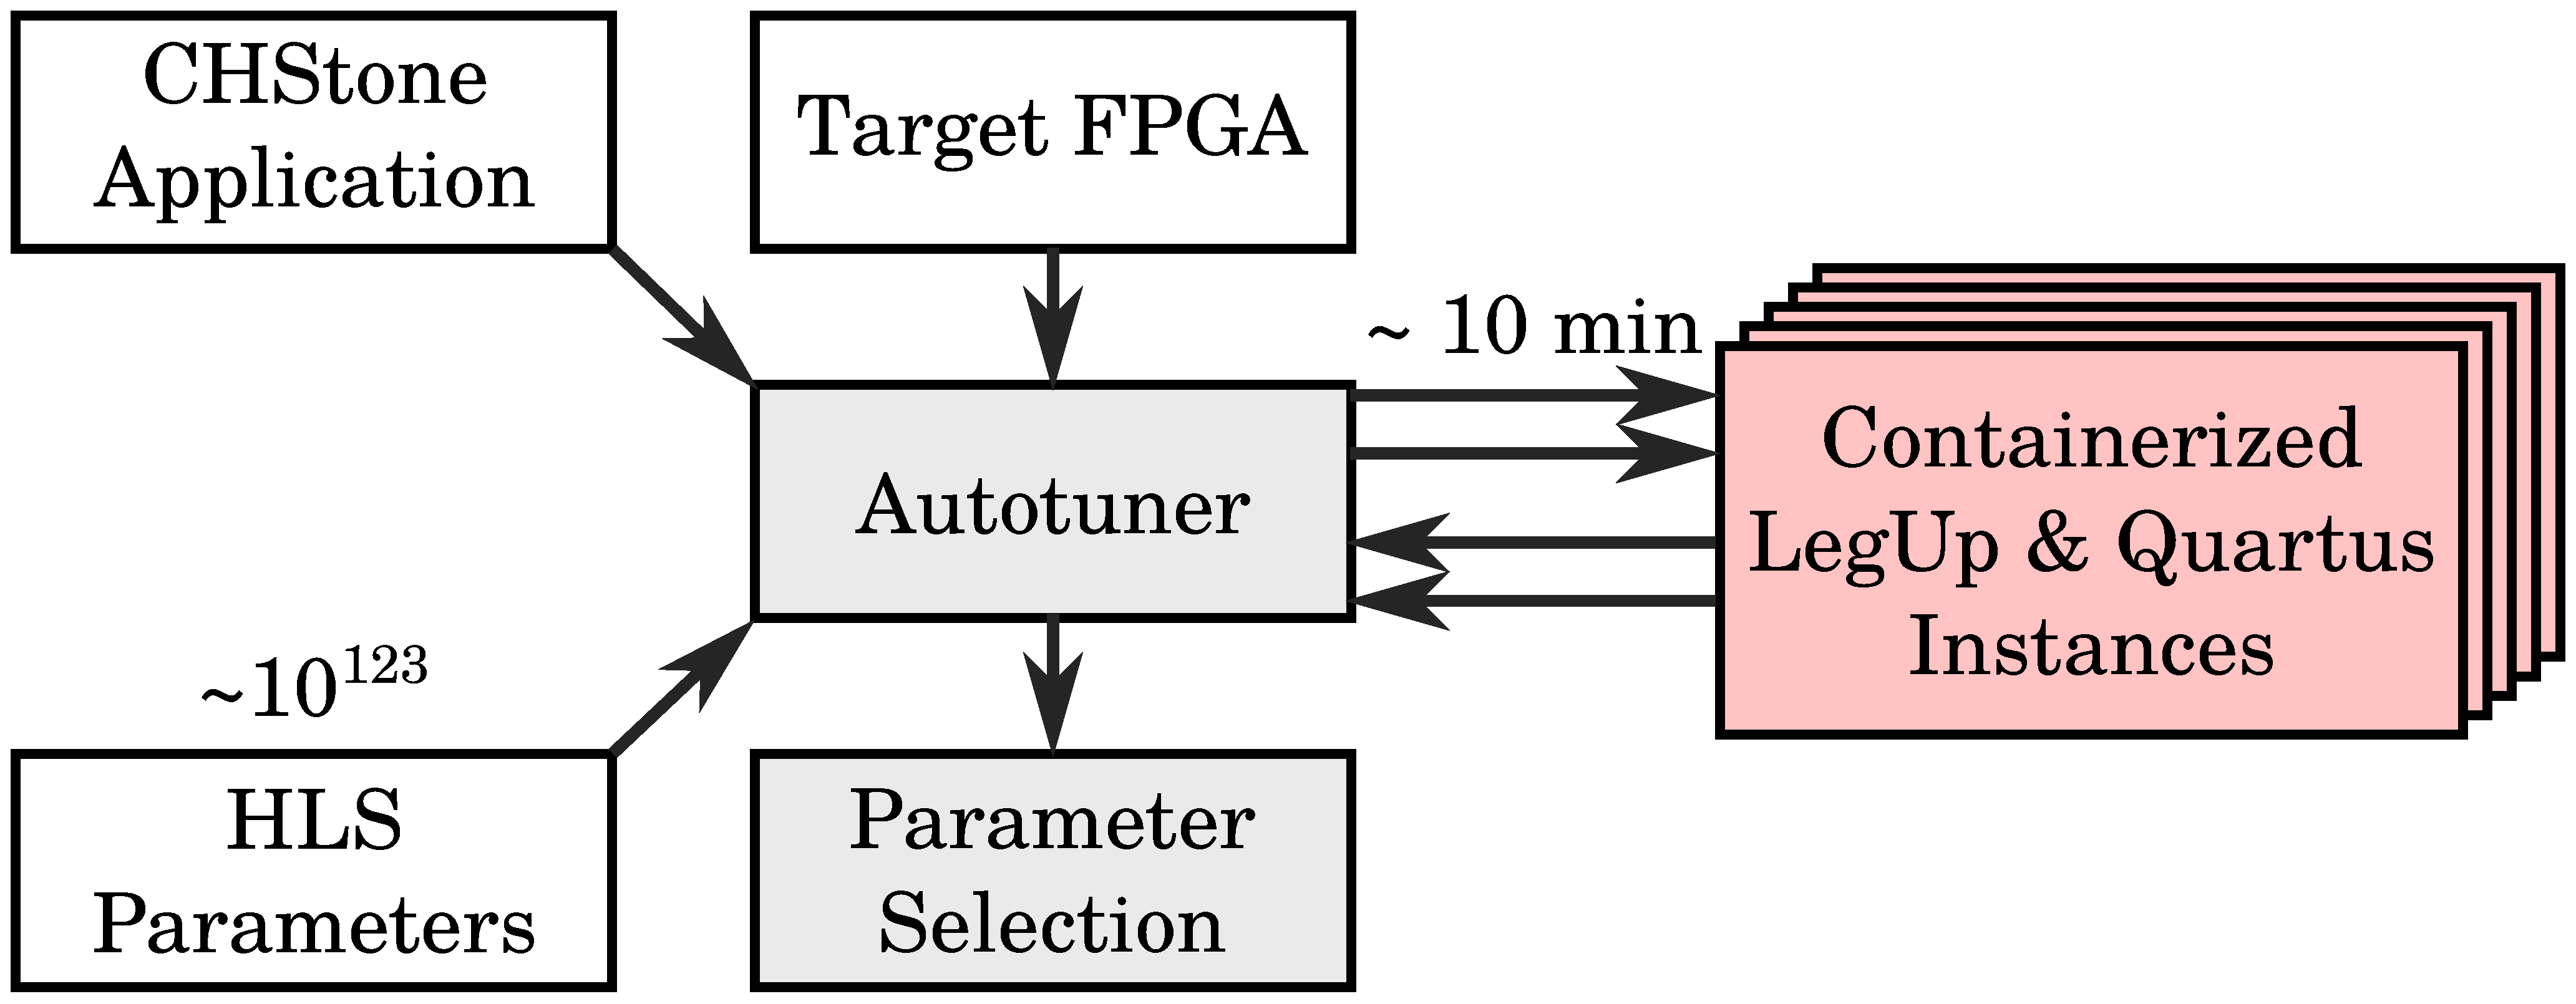
\includegraphics[width=0.6\columnwidth]{fpga_docker_tuner}
    \caption{Autotuner Setup}
    \label{fig:autotuner}
\end{figure}

Figure \ref{fig:autotuner} shows our setup using Docker containers running
LegUp and Quartus. This virtualized setup enabled the portable installation of
dependencies and can be used to run experiments in distributed environments.
The arrows coming from the autotuner to the containers represent the flow of
new configurations generated by search techniques, and the arrows coming from
the containers to the autotuner represent the flow of measurements for a set of
parameters. For CHStone applications the measurement process takes
approximately $10$ minutes to complete, and the majority of this time is spent
in Quartus's synthesis, mapping and place \& route.

\subsubsection{High-Level Synthesis Parameters}

We selected an extensive set of LegUp High-Level Synthesis parameters, shown
partially in Table \ref{tab:params}. Each parameter in the first two rows of
Table \ref{tab:params} has an $8$, $16$, $32$ and $64$ bit variant.
\textit{Operation Latency} parameters define the number of clock cycles
required to complete a given operation when compiled with LegUp.
\textit{Zero-latency} operations can be performed in a single clock cycle.
\textit{Resource Constraint} parameters define the number of times a given
operation can be performed in a clock cycle.  \textit{Boolean or Multi-Valued}
parameters are used to set various advanced configurations. For example, the
\textbf{\texttt{\small{enable\_pattern\_sharing}}} parameter can be set to
enable resource sharing for patterns of computational operators, as is
described by Hadjis \emph{et al.}~\cite{hadjis2012impact}.  For a complete list
and description of each parameter, please refer to LegUp's official
documentation~\footnote{\url{http://legup.eecg.utoronto.ca/docs/4.0} [Accessed
in 18/07/2017]}.

\begin{table}[htpb]
\centering
\begin{tabular}{@{}p{0.10\columnwidth}p{0.84\columnwidth}@{}}
\toprule
Type & \multicolumn{1}{c}{Parameters} \\ \midrule
\parbox[t]{0.10\columnwidth}{\scriptsize{Operation \\ Latency}} & \scriptsize{\texttt{\textbf{altfp\_}[divide, truncate, fptosi, add, subtract, multiply, extend, sitofp], \textbf{unsigned\_}[multiply, divide, add, modulus], \textbf{signed\_}[modulus, divide, multiply, add, \textbf{comp\_}[o, u]], [local\_mem, mem]\textbf{\_dual\_port}, \textbf{reg}}} \\
%\addlinespace{}
\parbox[t]{0.10\columnwidth}{\scriptsize{Resource Constraint}} & \scriptsize{\texttt{\textbf{signed\_}[divide, multiply, modulus, add], \textbf{altfp\_}[multiply, add, subtract, divide], \textbf{unsigned\_}[modulus, multiply, add, divide], [shared\_mem, mem]\textbf{\_dual\_port}}} \\
%\addlinespace{}
\parbox[t]{0.10\columnwidth}{\scriptsize{Boolean~or Multi-value}} & \scriptsize{\texttt{\textbf{pattern\_share\_}[add, shift, sub, bitops], \textbf{sdc\_}[multipump, no\_chaining, priority], \textbf{pipeline\_}[resource\_sharing, all], \textbf{ps\_}[min\_size, min\_width, max\_size, bit\_diff\_threshold], \textbf{mb\_}[minimize\_hw, max\_back\_passes], \textbf{no\_roms}, \textbf{multiplier\_no\_chain}, \textbf{dont\_chain\_get\_elem\_ptr}, \textbf{clock\_period}, \textbf{no\_loop\_pipelining}, \textbf{incremental\_sdc}, \textbf{disable\_reg\_sharing}, \textbf{set\_combine\_basicblock}, \textbf{enable\_pattern\_sharing}, \textbf{multipumping}, \textbf{dual\_port\_binding}, \textbf{modulo\_scheduler}, \textbf{explicit\_lpm\_mults}}} \\ \bottomrule
%%\addlinespace{}
\end{tabular}
\caption{Subset of All Autotuned LegUP HLS Parameters}
\label{tab:params}
\end{table}

\subsubsection{Autotuning Metrics}
\label{sec:metrics}

To obtain values for hardware metrics we needed to perform the synthesis,
mapping and place \& route steps. We used Quartus to do so, and selected 8
hardware metrics reported by Quartus to compose our cost or fitness function.
From the fitter summary we obtained 6 metrics. \textit{Logic Utilization}
(\textit{LUT}) measures the number of logic elements and is composed of
Adaptive Look-Up Table (ALUTs), memory ALUTs, logic registers or dedicated
logic registers.  The \textit{Registers} (\textit{Regs.}), \textit{Virtual
Pins} (\textit{Pins}), \textit{Block Memory Bits} (\textit{Blocks}),
\textit{RAM Blocks} (\textit{BRAM}) and \textit{DSP Blocks} (\textit{DSP})
metrics measure the usage of the resources indicated by their names.

From the timing analysis we obtained the \textit{Cycles} and \textit{FMax}
metrics, used to compute the \textit{Wall-Clock Time} metric. This metric
composed the cost function, but \textit{Cycles} and \textit{FMax} were not
individually used. We chose to do that because all of our hardware metrics
needed to be minimized except for \textit{FMax}, and computing
\textit{Wall-Clock Time} instead solved that restriction.  The
\textit{Wall-Clock Time} $wct$ is computed by $wct = \text{\textit{Cycles}}
\times (\alpha / \text{\textit{FMax}})$, where $\alpha = 10^6$ because
\textit{FMax} is reported in MHz.

Equation \ref{eq:wnsm} describes the cost or fitness function used by our
autotuner to evaluate the sets of HLS parameters generated during tuning.  The
function $f(M, W)$ computes a \textit{Weighted Normalized Sum} (\textbf{WNS})
of the measured metrics $m_i \in M$, where $M$ was described previously.  The
weights $w_i \in W$ correspond to one of the scenarios in Table
\ref{tab:scenarios}. A value is computed for each metric $m_i$ in relation to
an initial value $m_{i}^{0}$ measured for each metric.  For a given set of
measurements $M_t$, a value of $f(M_t, W) = 1.0$ means that there was no
improvement relative to the starting HLS set. The objective of the autotuner is
to minimize $f(M, W)$.

\begin{align} \label{eq:wnsm}
    \mathlarger{f(M, W)} = \frac{\mathlarger{\mathlarger{\mathlarger{\sum}}}\limits_{\substack{m_i \in M \\ w_i \in W}}{w_i\left(\dfrac{m_i}{m_{i}^{0}}\right)}}{\mathlarger{\mathlarger{\mathlarger{\sum}}}\limits_{w_i \in W}{w_i}}
\end{align}

\subsection{Experiments}
\label{sec:FPGAexp}

This section describes the optimization scenarios, the CHStone applications,
and the experimental settings.

\subsubsection{Optimization Scenarios}

Table \ref{tab:scenarios} shows the assigned weights in our $4$ optimization
scenarios. The \textit{Area}-targeting scenario assigns low weights to
wall-clock time metrics. The \textit{Performance \& Latency} scenario assigns
high weights to wall-clock time metrics and also to the number of registers
used.  The \textit{Performance} scenario assigns low weights to area metrics
and cycles, assigning a high weight only to frequency. The balanced scenario
assigns the same weight to every metric. The weights assigned to the metrics
that do not appear on Table \ref{tab:scenarios} are always $1$. The weights are
integers and powers of~$2$.

\begin{table}[htpb]
    \centering
    \begin{tabular}{@{}lcccc@{}}
        \toprule
        Metric & \textit{Area} & \textit{Perf. \& Lat} & \textit{Performance} & \textit{Balanced} \\ \midrule
        \textit{LUT} & \cellcolor[HTML]{9B94B6} High & \cellcolor[HTML]{DD9583} Low & \cellcolor[HTML]{DD9583} Low & \cellcolor[HTML]{E3DBB3} Medium \\
        \textit{Registers} & \cellcolor[HTML]{9B94B6} High & \cellcolor[HTML]{9B94B6} High & \cellcolor[HTML]{E3DBB3} Medium & \cellcolor[HTML]{E3DBB3} Medium \\
        \textit{BRAMs} & \cellcolor[HTML]{9B94B6} High & \cellcolor[HTML]{DD9583} Low & \cellcolor[HTML]{DD9583} Low & \cellcolor[HTML]{E3DBB3} Medium \\
        \textit{DSPs} & \cellcolor[HTML]{9B94B6} High & \cellcolor[HTML]{DD9583} Low & \cellcolor[HTML]{DD9583} Low & \cellcolor[HTML]{E3DBB3} Medium \\
        \textit{FMax} & \cellcolor[HTML]{DD9583} Low & \cellcolor[HTML]{9B94B6} High & \cellcolor[HTML]{9B94B6} High & \cellcolor[HTML]{E3DBB3} Medium \\
        \textit{Cycles} & \cellcolor[HTML]{DD9583} Low & \cellcolor[HTML]{9B94B6} High & \cellcolor[HTML]{DD9583} Low & \cellcolor[HTML]{E3DBB3} Medium \\ \bottomrule
    \end{tabular}
    \caption{Weights for Optimization Scenarios \\ (\textit{High} $= 8$, \textit{Medium} $= 4$, \textit{Low} $= 2$)}
    \label{tab:scenarios}
    %\addlinespace
\end{table}

We compared results when starting from a \textit{default} configuration with
the results when starting at a \textit{random} set of parameters. The default
configuration for the StratixV was provided by LegUp and the comparison was
performed in the \textit{Balanced} optimization scenario.

\subsubsection{Applications}

To test and validate our autotuner we used 11 applications from the CHStone HLS
benchmark suite~\cite{hara2008chstone}. CHStone applications are implemented in
the C language and contain inputs and previously computed outputs, allowing for
correctness checks to be performed for all applications.

\begin{table}[htpb]
\centering
\begin{tabular}{@{}p{0.13\columnwidth}p{0.63\columnwidth}@{}}
\toprule
 Application & Short Description \\ \midrule
 blowfish & Symmetric-key block cypher \\
 aes & Advanced Encryption Algorithm (AES) \\
 adpcm & Adaptive Differential Pulse Code Modulation dec. and enc. \\
 sha & Secure Hash Algorithm (SHA) \\
 motion & Motion vector decoding from MPEG-2 \\
 mips & Simplified MIPS processor \\
 gsm & Predictive coding analysis of systems for mobile comms. \\
 dfsin & Sine function for double-precision floating-point numbers \\
 dfmul & Double-precision floating-point multiplication \\
 dfdiv & Double-precision floating-point division \\
 dfadd & Double-precision floating-point addition \\ \bottomrule
%% \addlinespace{}
\end{tabular}
\caption{Autotuned CHStone Applications}
\label{tab:chstone}
\end{table}

Table \ref{tab:chstone} provides short descriptions of the $11$ CHStone
applications we used. We were not able to compile the \textit{jpeg} CHStone
application, so did not use it.  All experiments targeted the \textit{Intel
StratixV 5SGXEA7N2F45C2} FPGA.

\subsubsection{Experiments}

We performed $10$ tuning runs of $1.5h$ for each application.  Section
\ref{sec:FPGAresults} presents the mean relative improvements for each application
and individual metric. The code needed to run the experiments and generate the
figures, as well as the implementation of the autotuner and all data we
generated, is open and hosted at
GitHub~\footnote{\url{https://github.com/phrb/legup-tuner} [Accessed in
18/07/2017]}.

The experimental settings included Docker for virtualization and
reproducibility, LegUp $v4.0$, Quartus Prime Standard Edition $v16.0$, and
CHStone. All experiments were performed on a machine with two Intel(R) Xeon(R)
CPU E5-2699 v3 with 18 x86\_64 cores each, and 503GB of RAM.  The instructions
and the code to reproduce the software experimental environment are open and
hosted at GitHub~\footnote{\url{https://github.com/phrb/legup-dockerfile}
[Accessed in 18/07/2017]}.

\subsection{Results}
\label{sec:FPGAresults}

This section presents summaries of the results from $10$ autotuning runs of
$1.5h$ in the scenarios from Table \ref{tab:scenarios}.  Results are presented
in \textit{heatmaps} where each row has one of the 11 CHStone applications in
Table \ref{tab:chstone} and each column has one of the 8 hardware metrics and
their \textit{Weighted Normalized Sum} (\textbf{WNS}) as described in Section
\ref{sec:metrics}.

Cells on heatmaps show the ratio of tuned to initial values of a hardware
metric in a CHStone application, averaged over 10 autotuning runs. The
objective of the autotuner is to minimize all hardware metrics except for
\textit{FMax}.  To create a consistent presentation of our data in the heatmaps
we inverted the ratios for \textit{FMax} so that cell values less than $1.0$
always mean a better metric value.  Heatmaps are also colored so that darker
blues mean better values and darker reds mean worse values in relation to the
starting point.

\begin{figure}[htpb]
    \centering
    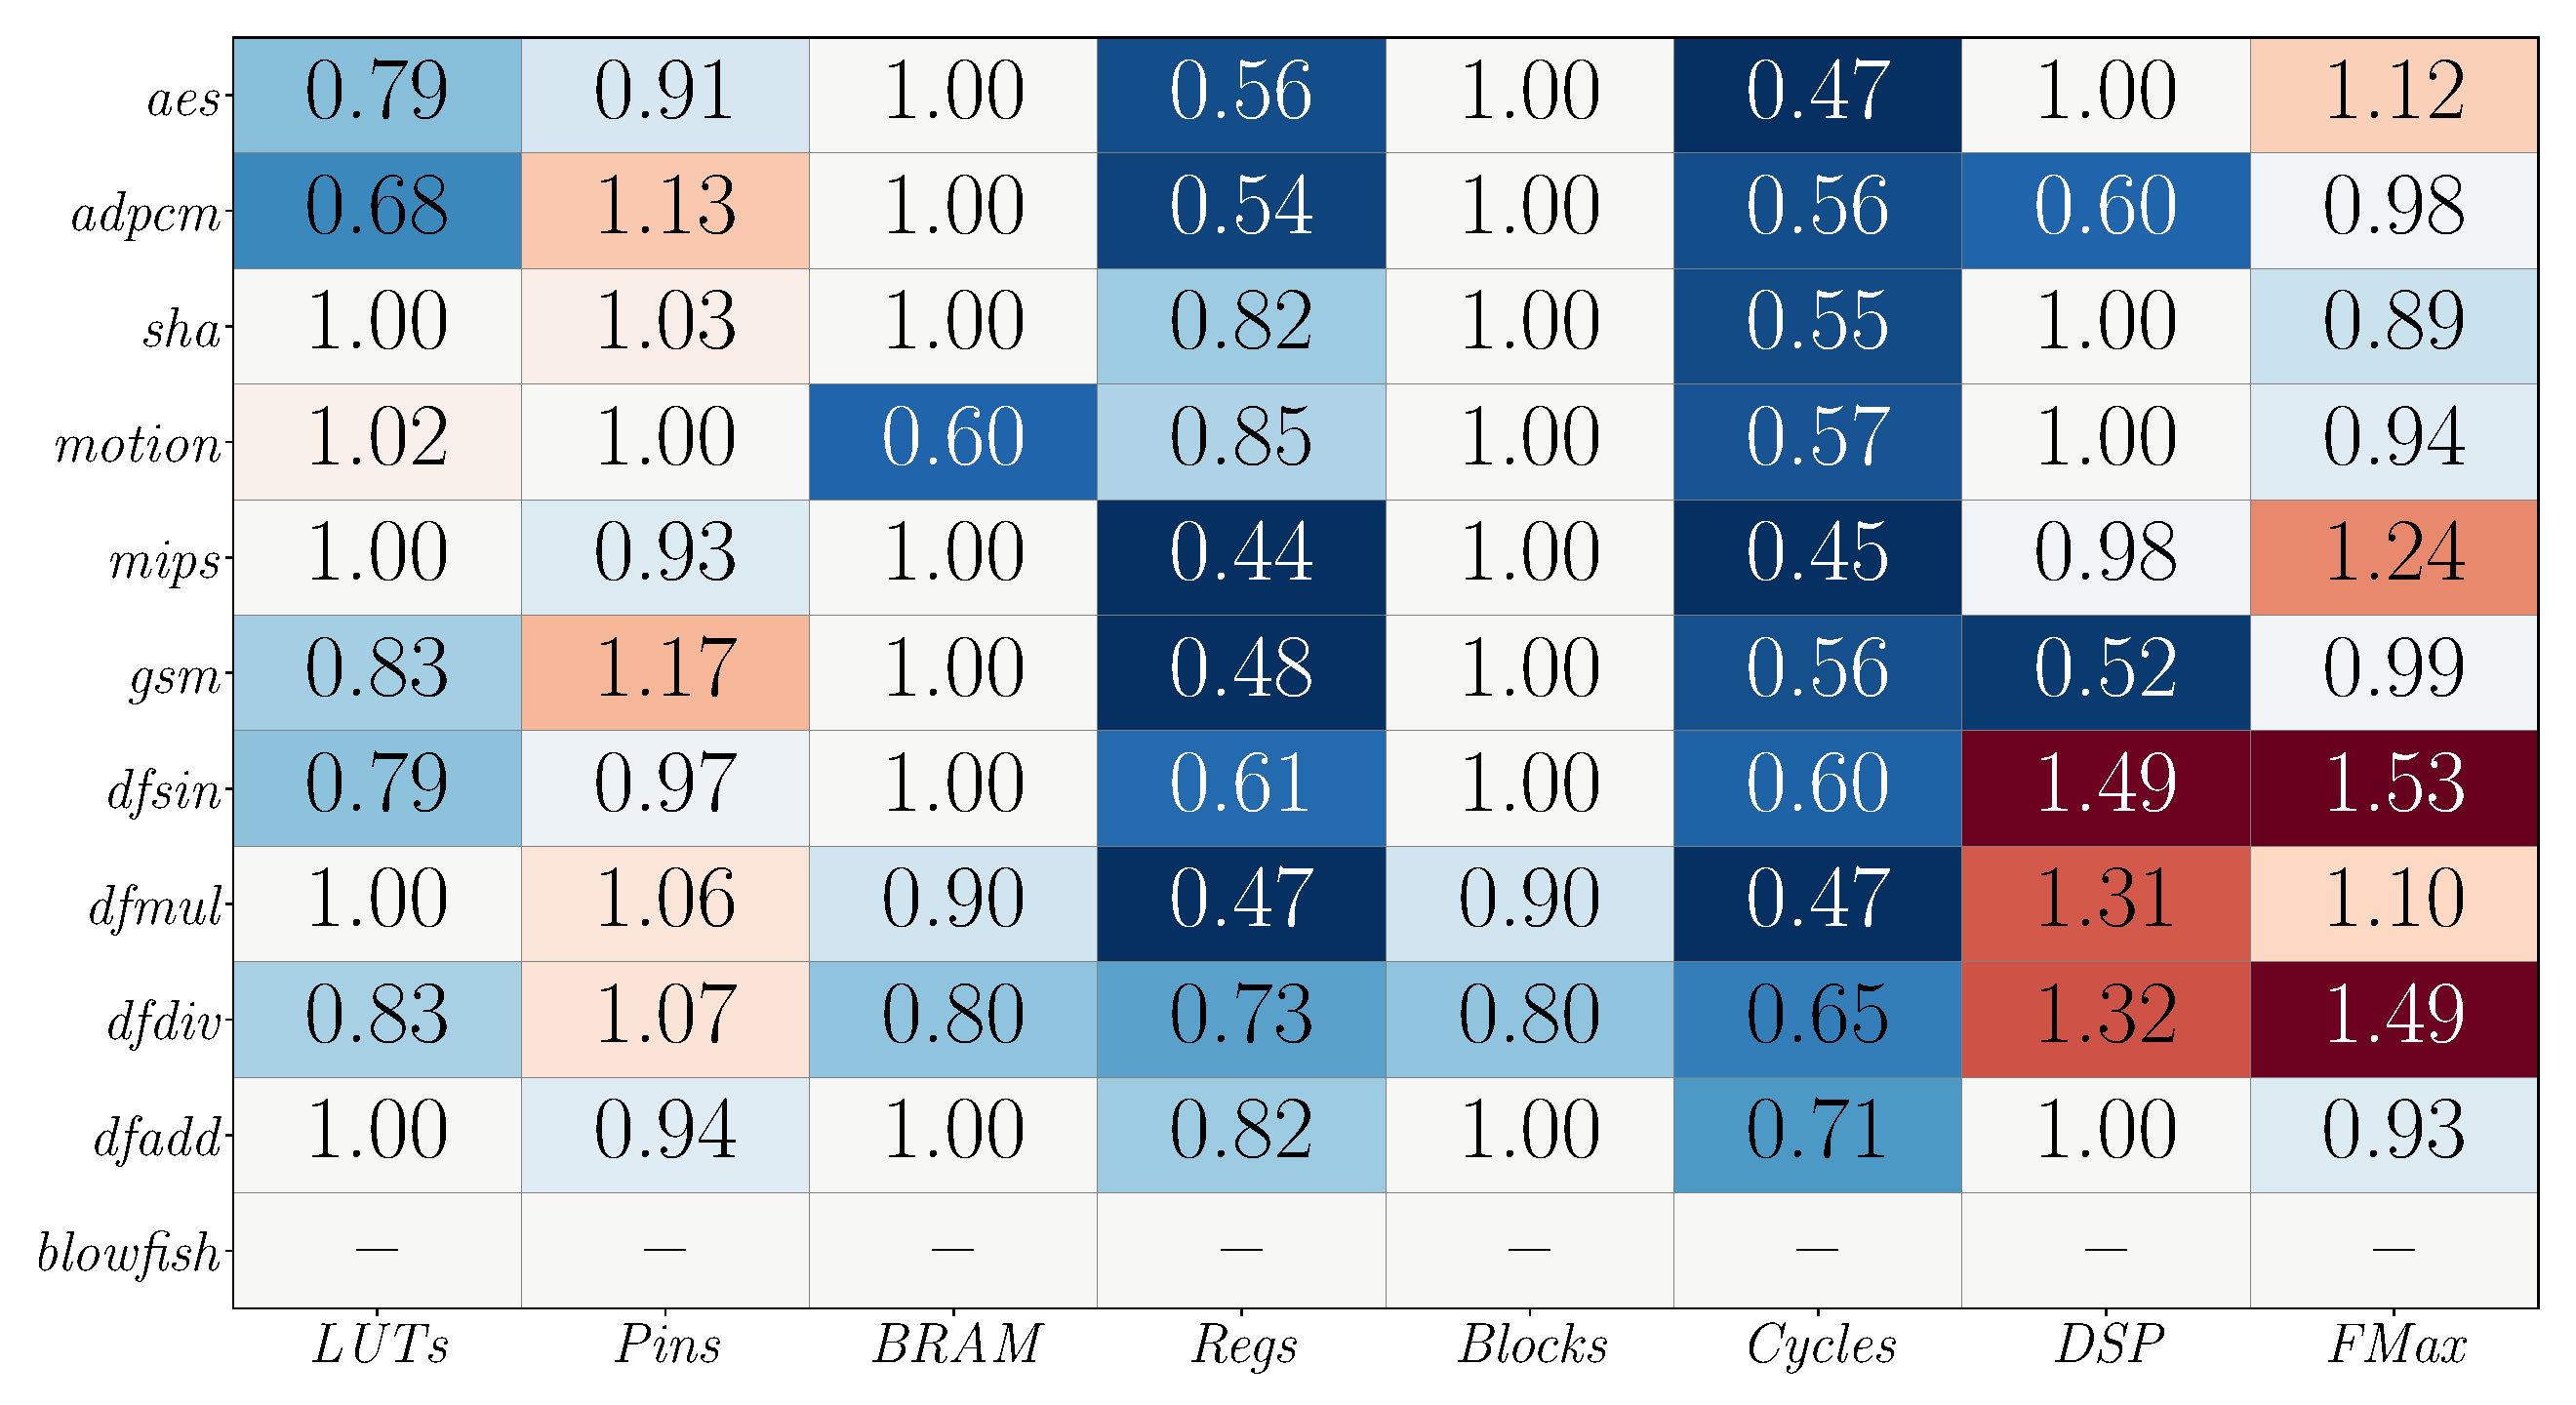
\includegraphics[width=0.5\columnwidth]{heatmap_comp_stratixV}
    \caption{Comparison of the absolute values for Random and Default starting points in the Balanced scenario}
    \label{fig:comp}
\end{figure}

Figure \ref{fig:comp} compares the ratios of absolute values for each hardware
metric for \textit{Default} and \textit{Random} starts, in the
\textit{Balanced} scenario.  Cell values less than $1.0$ mean that the
\textit{Default} start achieved smaller absolute values that the
\textit{Random} start.  Values of ``--'' mean that the \textit{Default} start
could not find a set of HLS parameters that produced a valid output during any
of the $1.5h$ tuning runs. The \textit{Default} start found better values for
most metrics.

The \textit{Random} start found better values for \textit{DSP}, \textit{Pins}
and \textit{FMax} for some applications. For example, it found values $49\%$
smaller, $6\%$ smaller and $53\%$ larger for \textit{DSP}, \textit{Pins} and
\textit{FMax}, respectively, for the \textit{dfsin} application. The
\textit{Default} start found better values for \textit{Regs} and
\textit{Cycles} for all applications. For example, it found values $53\%$
smaller for \textit{Regs} and \textit{Cycles} for the \textit{dfmul}
application, and $56\%$ and $55\%$ smaller for \textit{Regs} and
\textit{Cycles}, respectively, for the \textit{mips} application.

We believe that the \textit{Random} start found worst values in most cases
because of the size of the search space. It is important that autotuners use
default starting points specific to a given application and board.  The
remaining results in this Section used the \textit{Default} starting point
provided by LegUp.

Figure \ref{fig:balanced} shows the results for the \textit{Balanced} scenario.
These results are the baseline for evaluating the autotuner in other scenarios,
since all metrics had the same weight.  The optimization target was the
\textit{Weighted Normalized Sum} (\textbf{WNS}) of hardware metrics, but we
were also interested in the changes in other metrics as their relative weights
changed. In the \textit{Balanced} scenario we expected to see smaller
improvements of \textbf{WNS} due to the competition of concurrent improvements
on every metric.

The autotuner found values of \textbf{WNS} $16\%$ smaller for \textit{adpcm}
and \textit{dfdiv}, and $15\%$ smaller for \textit{dfmul}.  Even on the
\textit{Balanced} scenario it is possible to see that some metrics decreased
while others decreased consistently over the 10 tuning runs. \textit{FMax} and
\textit{DSP} had the larger improvements for most applications, for example,
$51\%$ greater \textit{FMax} in \textit{adpcm} and $69\%$ smaller \textit{DSP}
in \textit{dfmul}.  \textit{Cycles}, \textit{Regs} and \textit{Pins} had the
worst results in this scenario, with $34\%$ larger \textit{Cycles} in
\textit{dfdiv}, $15\%$ larger \textit{Regs} in \textit{dfdiv} and $17\%$ larger
\textit{Pins} in \textit{gsm}.  Other metrics had smaller improvements or no
improvements at all in most applications.

\begin{figure}[htpb]
    \begin{minipage}{.48\textwidth}
        \centering
        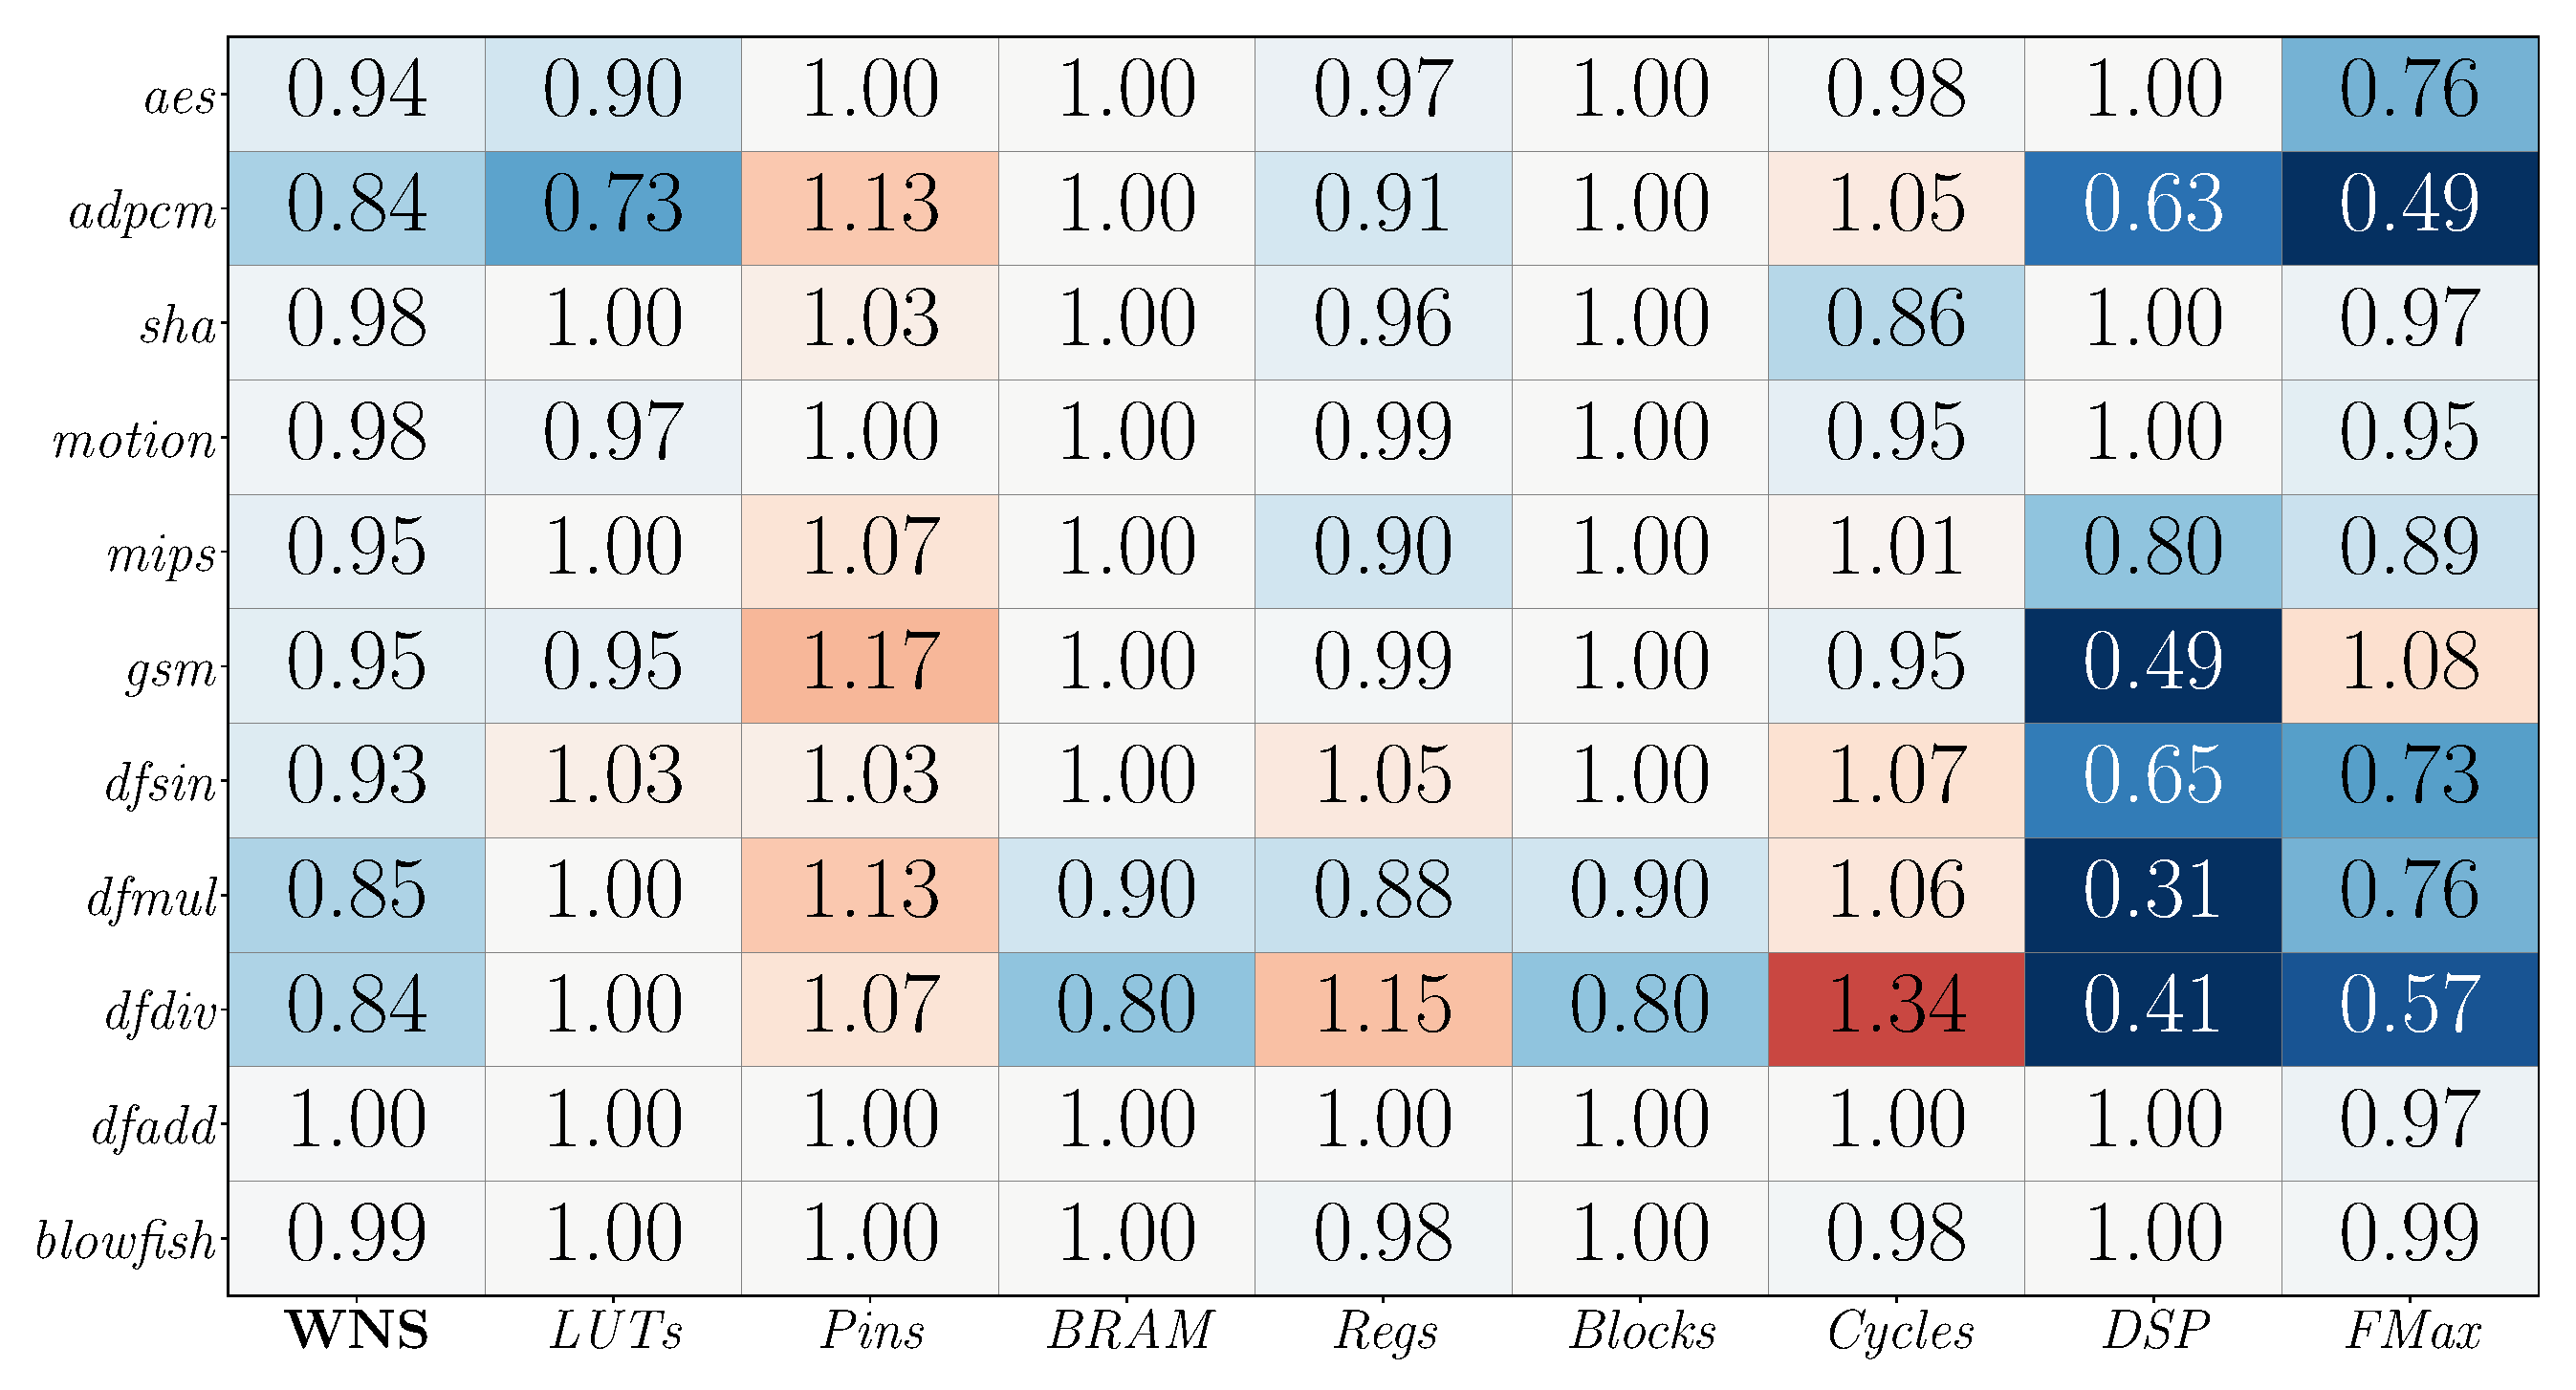
\includegraphics[width=\columnwidth]{heatmap_default_stratixV}
        \caption{Relative improvement for all metrics in the \textit{Balanced}
        scenario}
        \label{fig:balanced}
    \end{minipage}%
    \hfill
    \begin{minipage}{.48\textwidth}
        \centering
        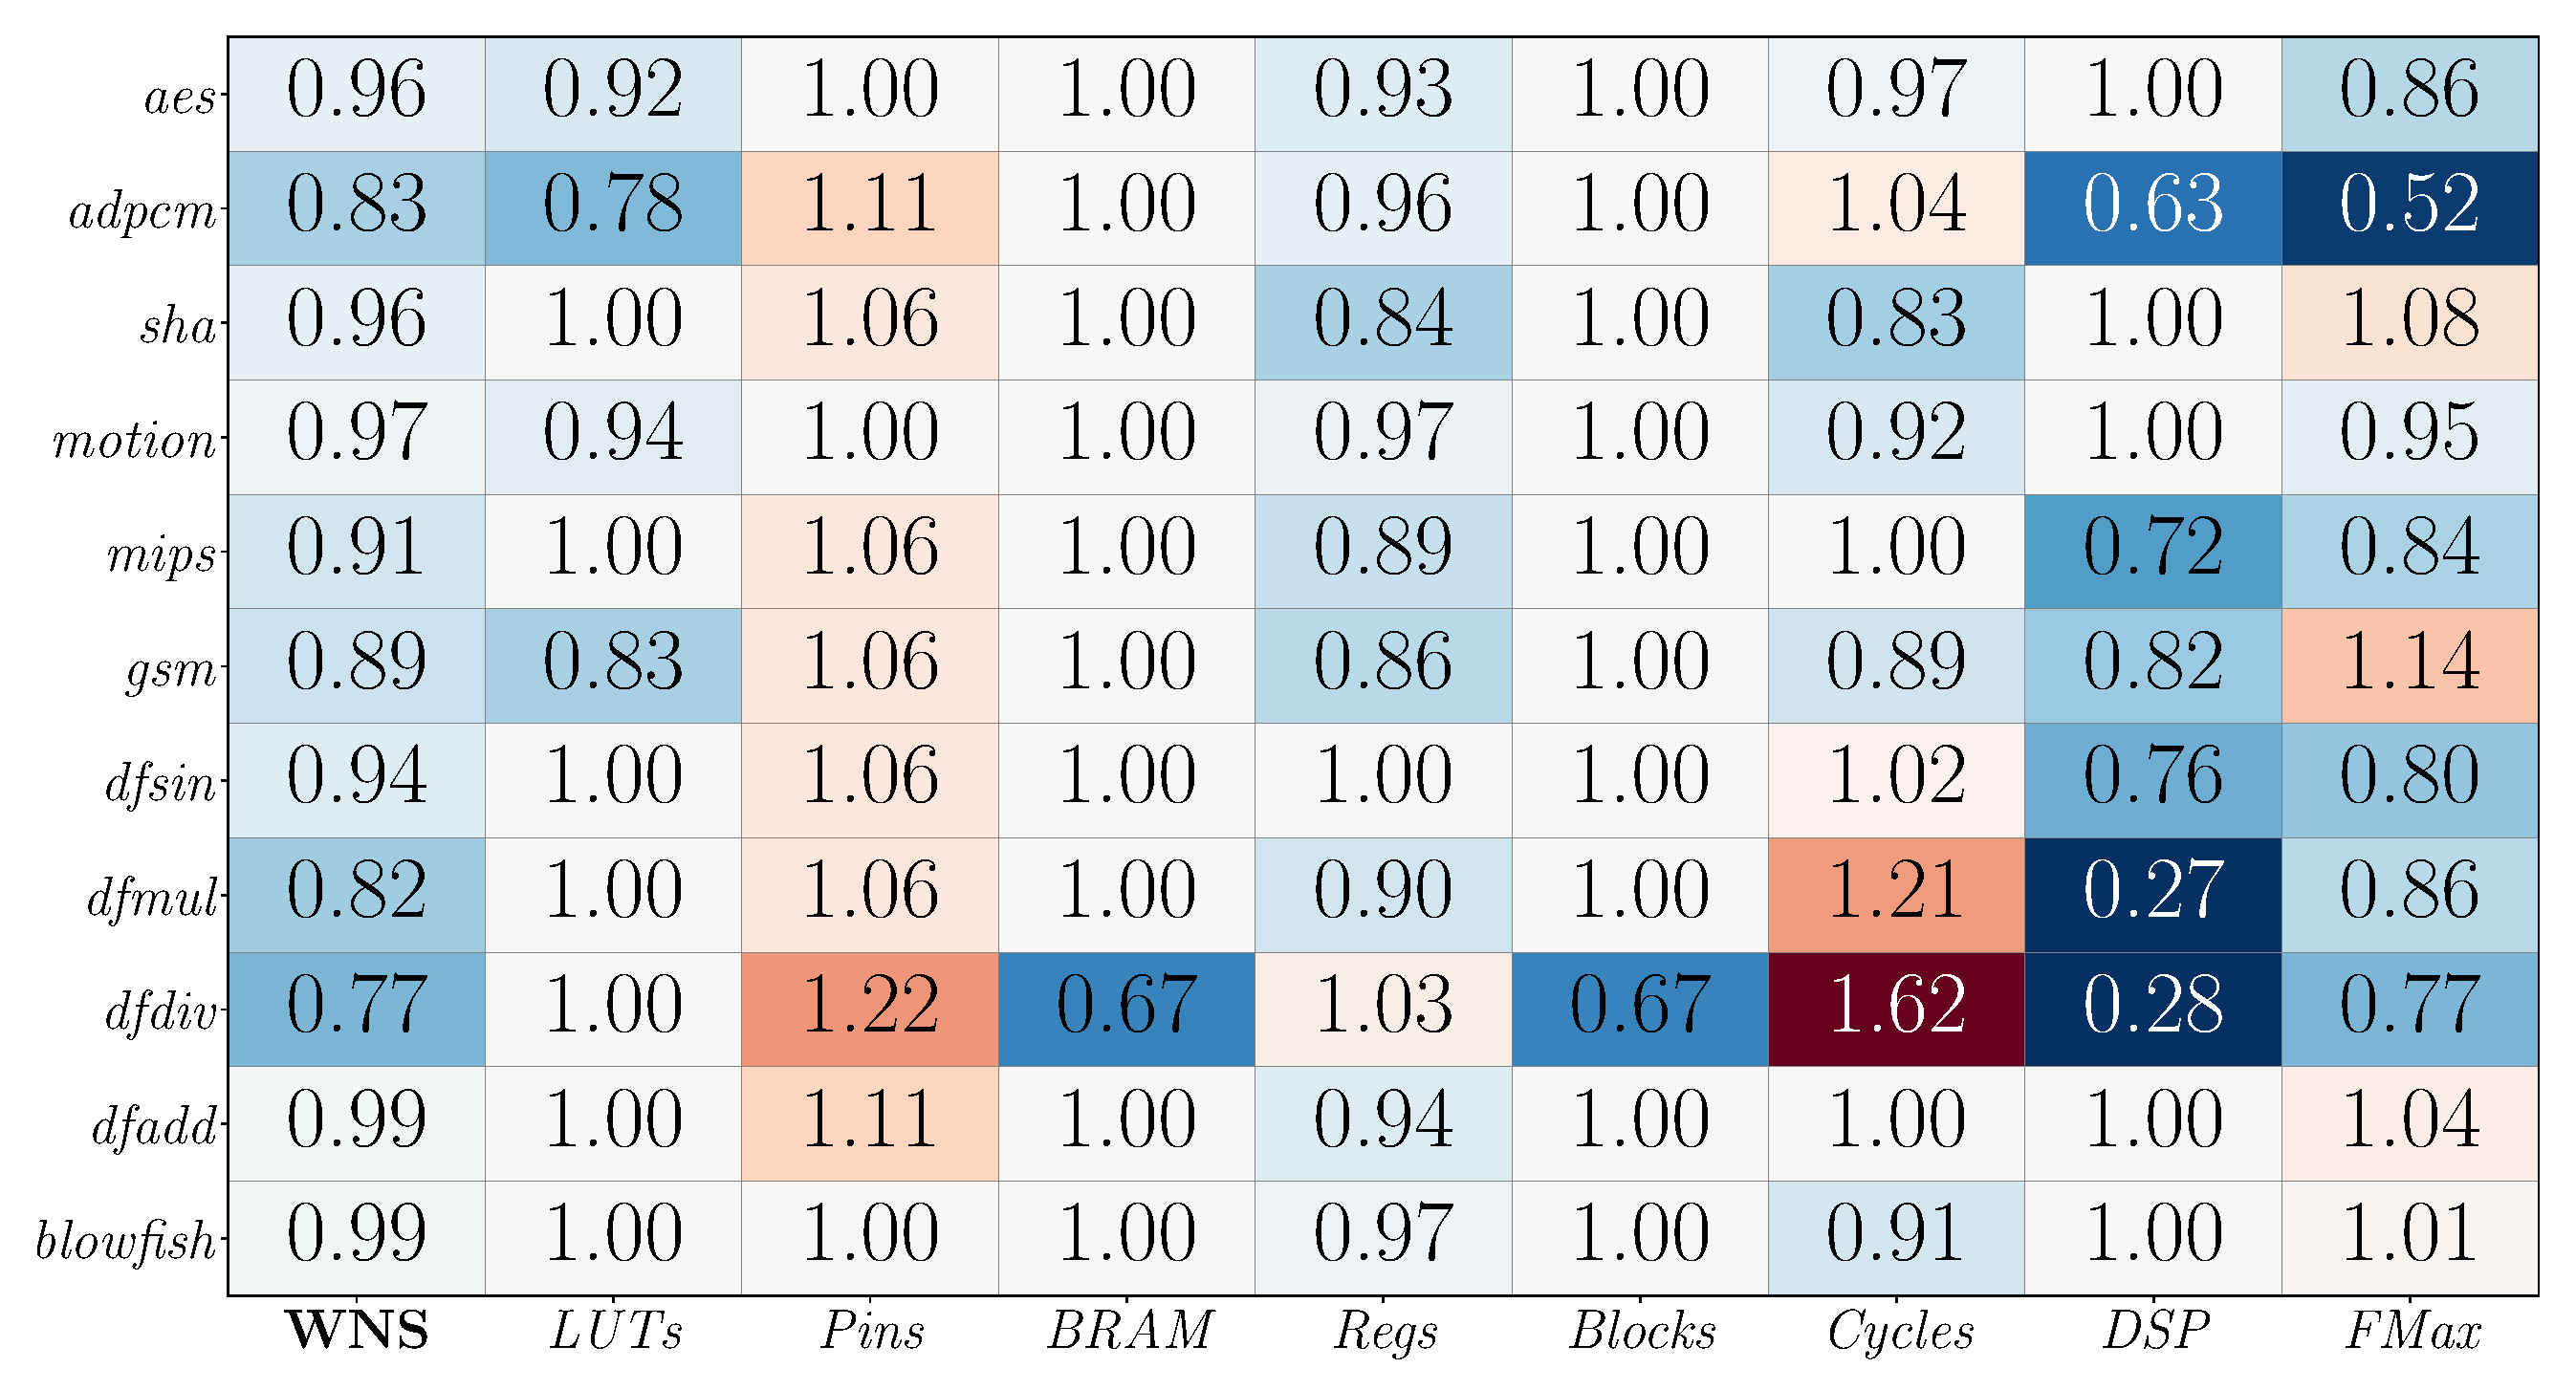
\includegraphics[width=\columnwidth]{heatmap_default_stratixV_area}
        \caption{Relative improvement for all metrics in the \textit{Area}
        scenario}
        \label{fig:area}
    \end{minipage}%
\end{figure}

Figure \ref{fig:area} shows the results for the \textit{Area} scenario.  We
believe that the greater coherence of optimization objectives is responsible
for the greater improvements of \textbf{WNS} in the following scenarios. The
autotuner found values of \textbf{WNS} $23\%$ smaller for \textit{dfdiv},
$18\%$ smaller for \textit{dfmul}, and smaller values overall in comparison
with the \textit{Balanced} scenario. Regarding individual metrics, the values
for \textit{FMax} were worse overall, with $14\%$ smaller \textit{FMax} in
\textit{gsm} and $62\%$ greater \textit{Cycles}, for example. As expected for
this scenario, metrics related to area had better improvements than in the
\textit{Balanced} scenario, with $73\%$ and $72\%$ smaller \textit{DSP} for
\textit{dfmul} and \textit{dfdiv} respectively, $33\%$ smaller \textit{Blocks}
and \textit{BRAM} in \textit{dfdiv} and smaller values overall for
\textit{Regs} and \textit{LUTs}.

Figure \ref{fig:perf} shows the results for the \textit{Performance} scenario.
The autotuner found values of \textbf{WNS} $23\%$ smaller for \textit{dfmul},
$19\%$ smaller for \textit{dfdiv}, and smaller values overall than in the
\textit{Balanced} scenario.  \textit{FMax} was the only metric with a
\textit{High} weight in this scenario, so most metrics had improvements close
overall to the \textit{Balanced} scenario.  The values for \textit{FMax} were
best overall, with better improvements in most applications. For example,
$41\%$, $30\%$, $44\%$ and $37\%$ greater \textit{FMax} in \textit{dfdiv},
\textit{dfmul}, \textit{dfsin} and \textit{aes} respectively.

\begin{figure}[htpb]
    \centering
    \begin{minipage}{.48\textwidth}
        \centering
        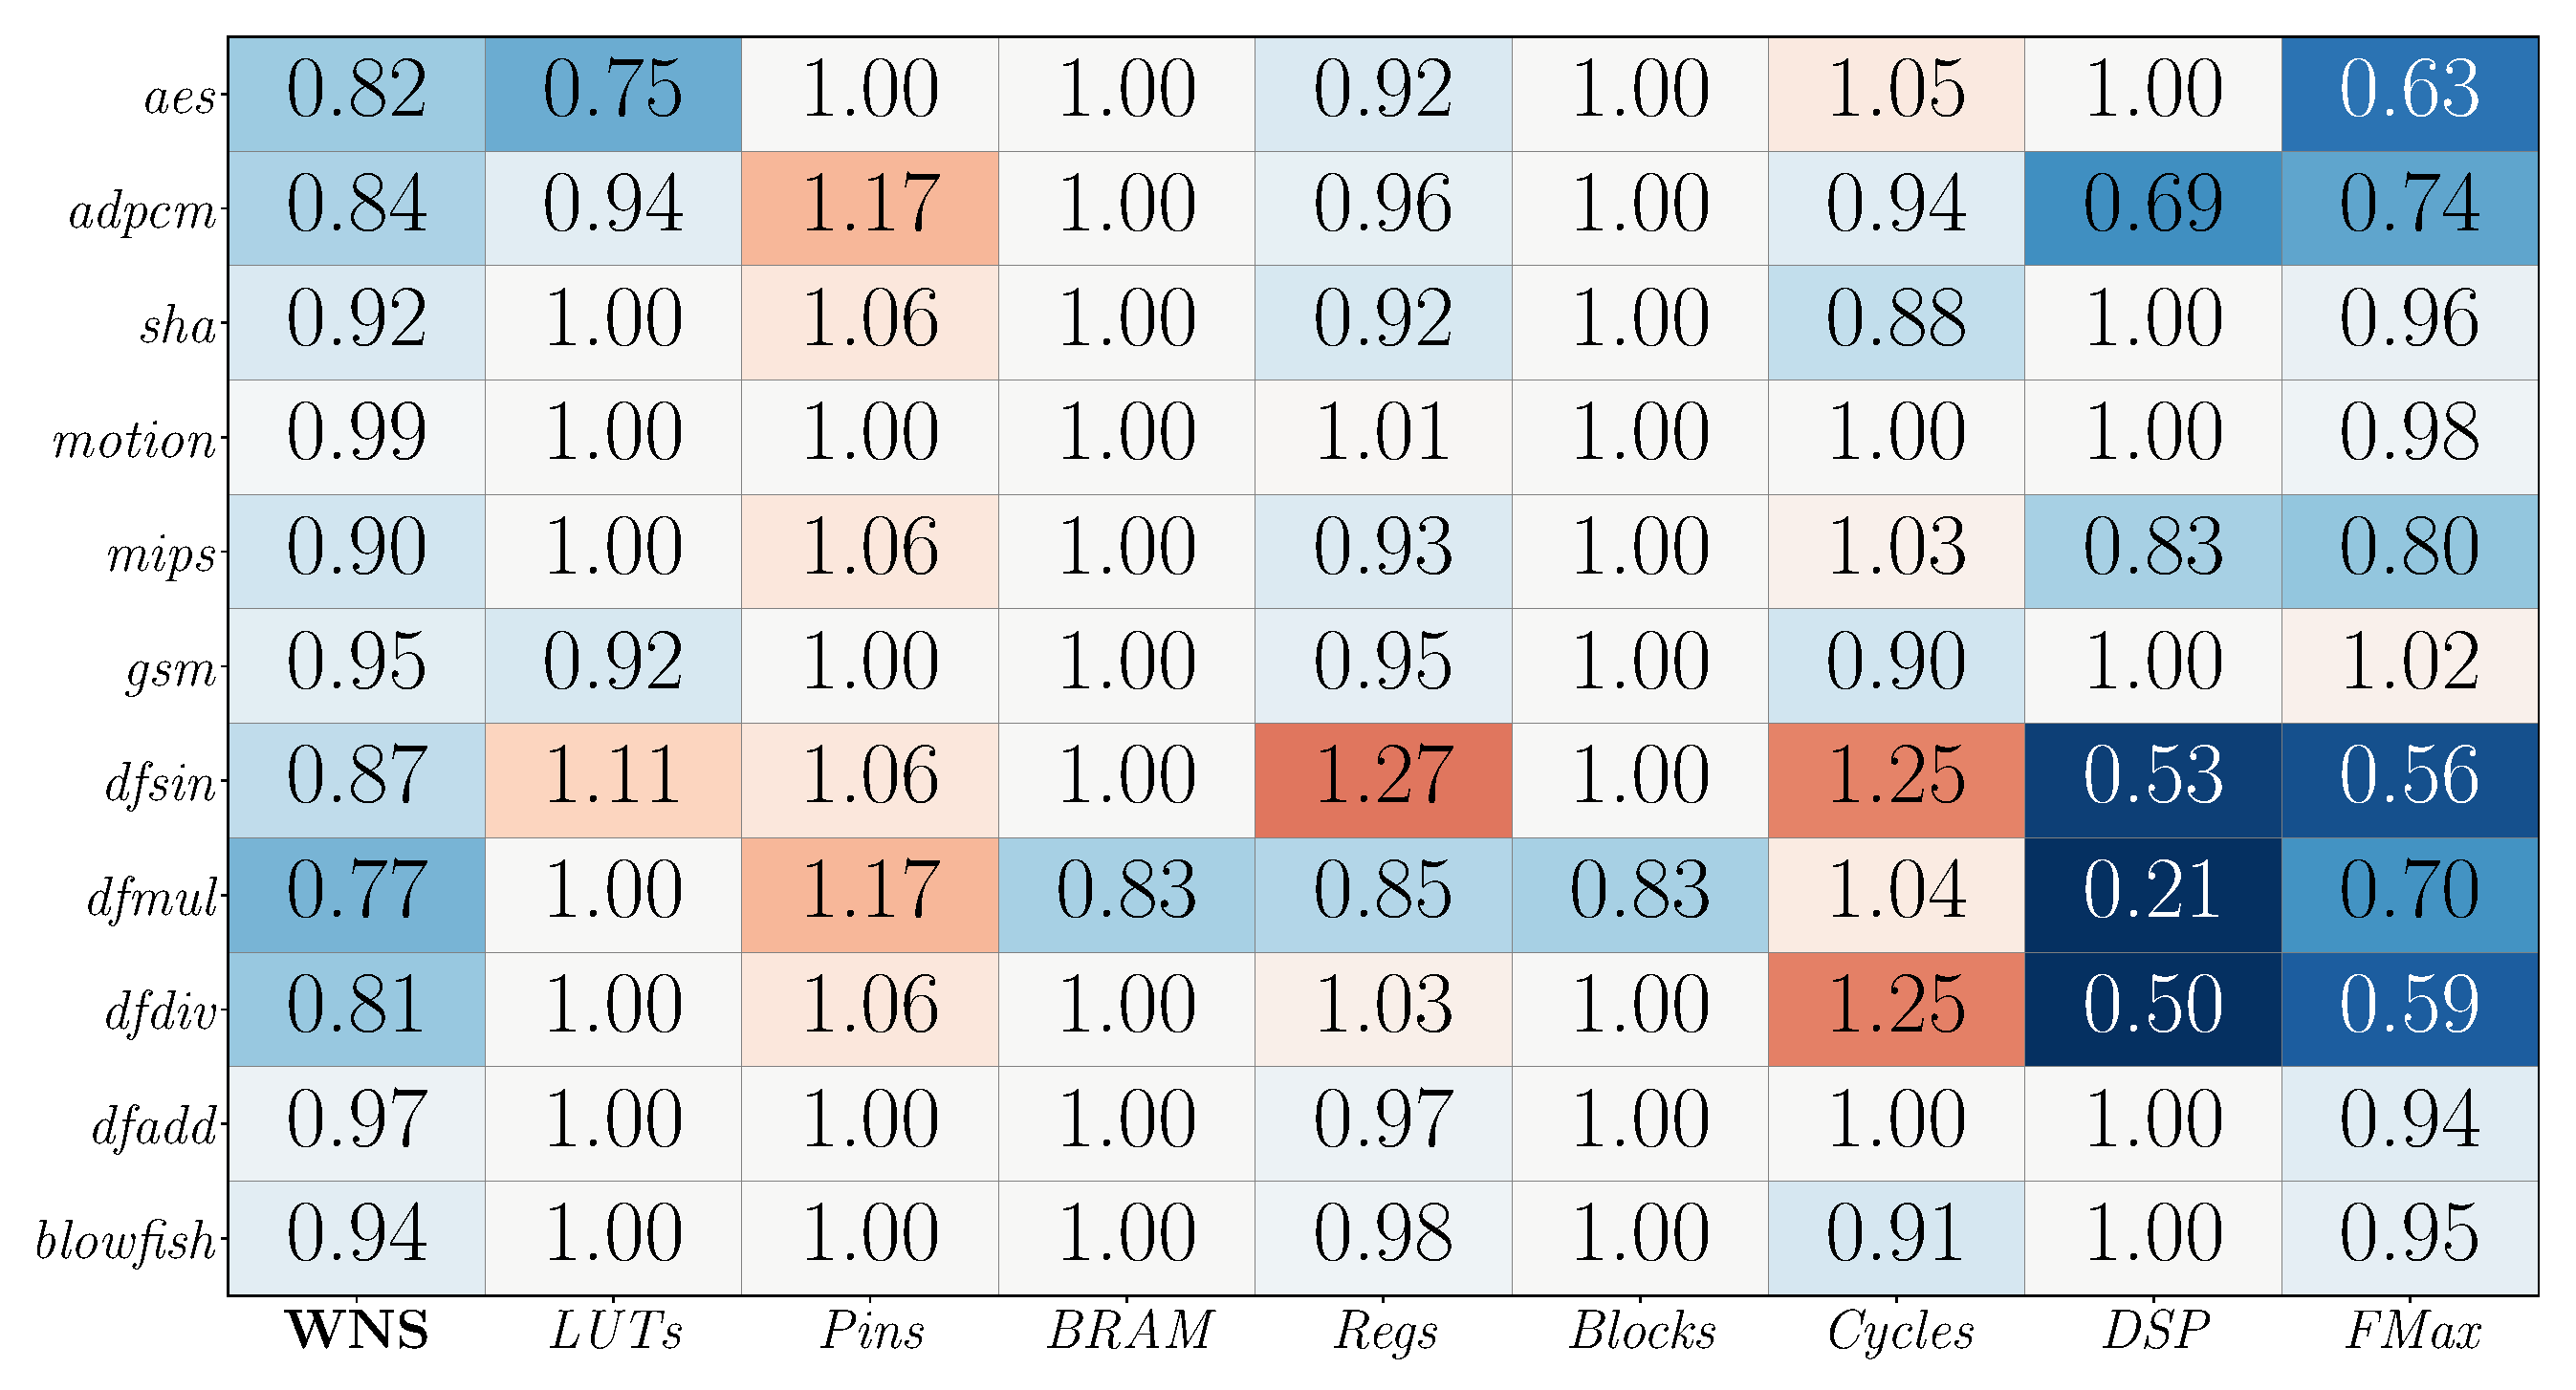
\includegraphics[width=\columnwidth]{heatmap_default_stratixV_perf}
        \caption{Relative improvement for all metrics in the
        \textit{Performance} scenario}
        \label{fig:perf}
    \end{minipage}%
    \hfill
    \begin{minipage}{.48\textwidth}
        \centering
        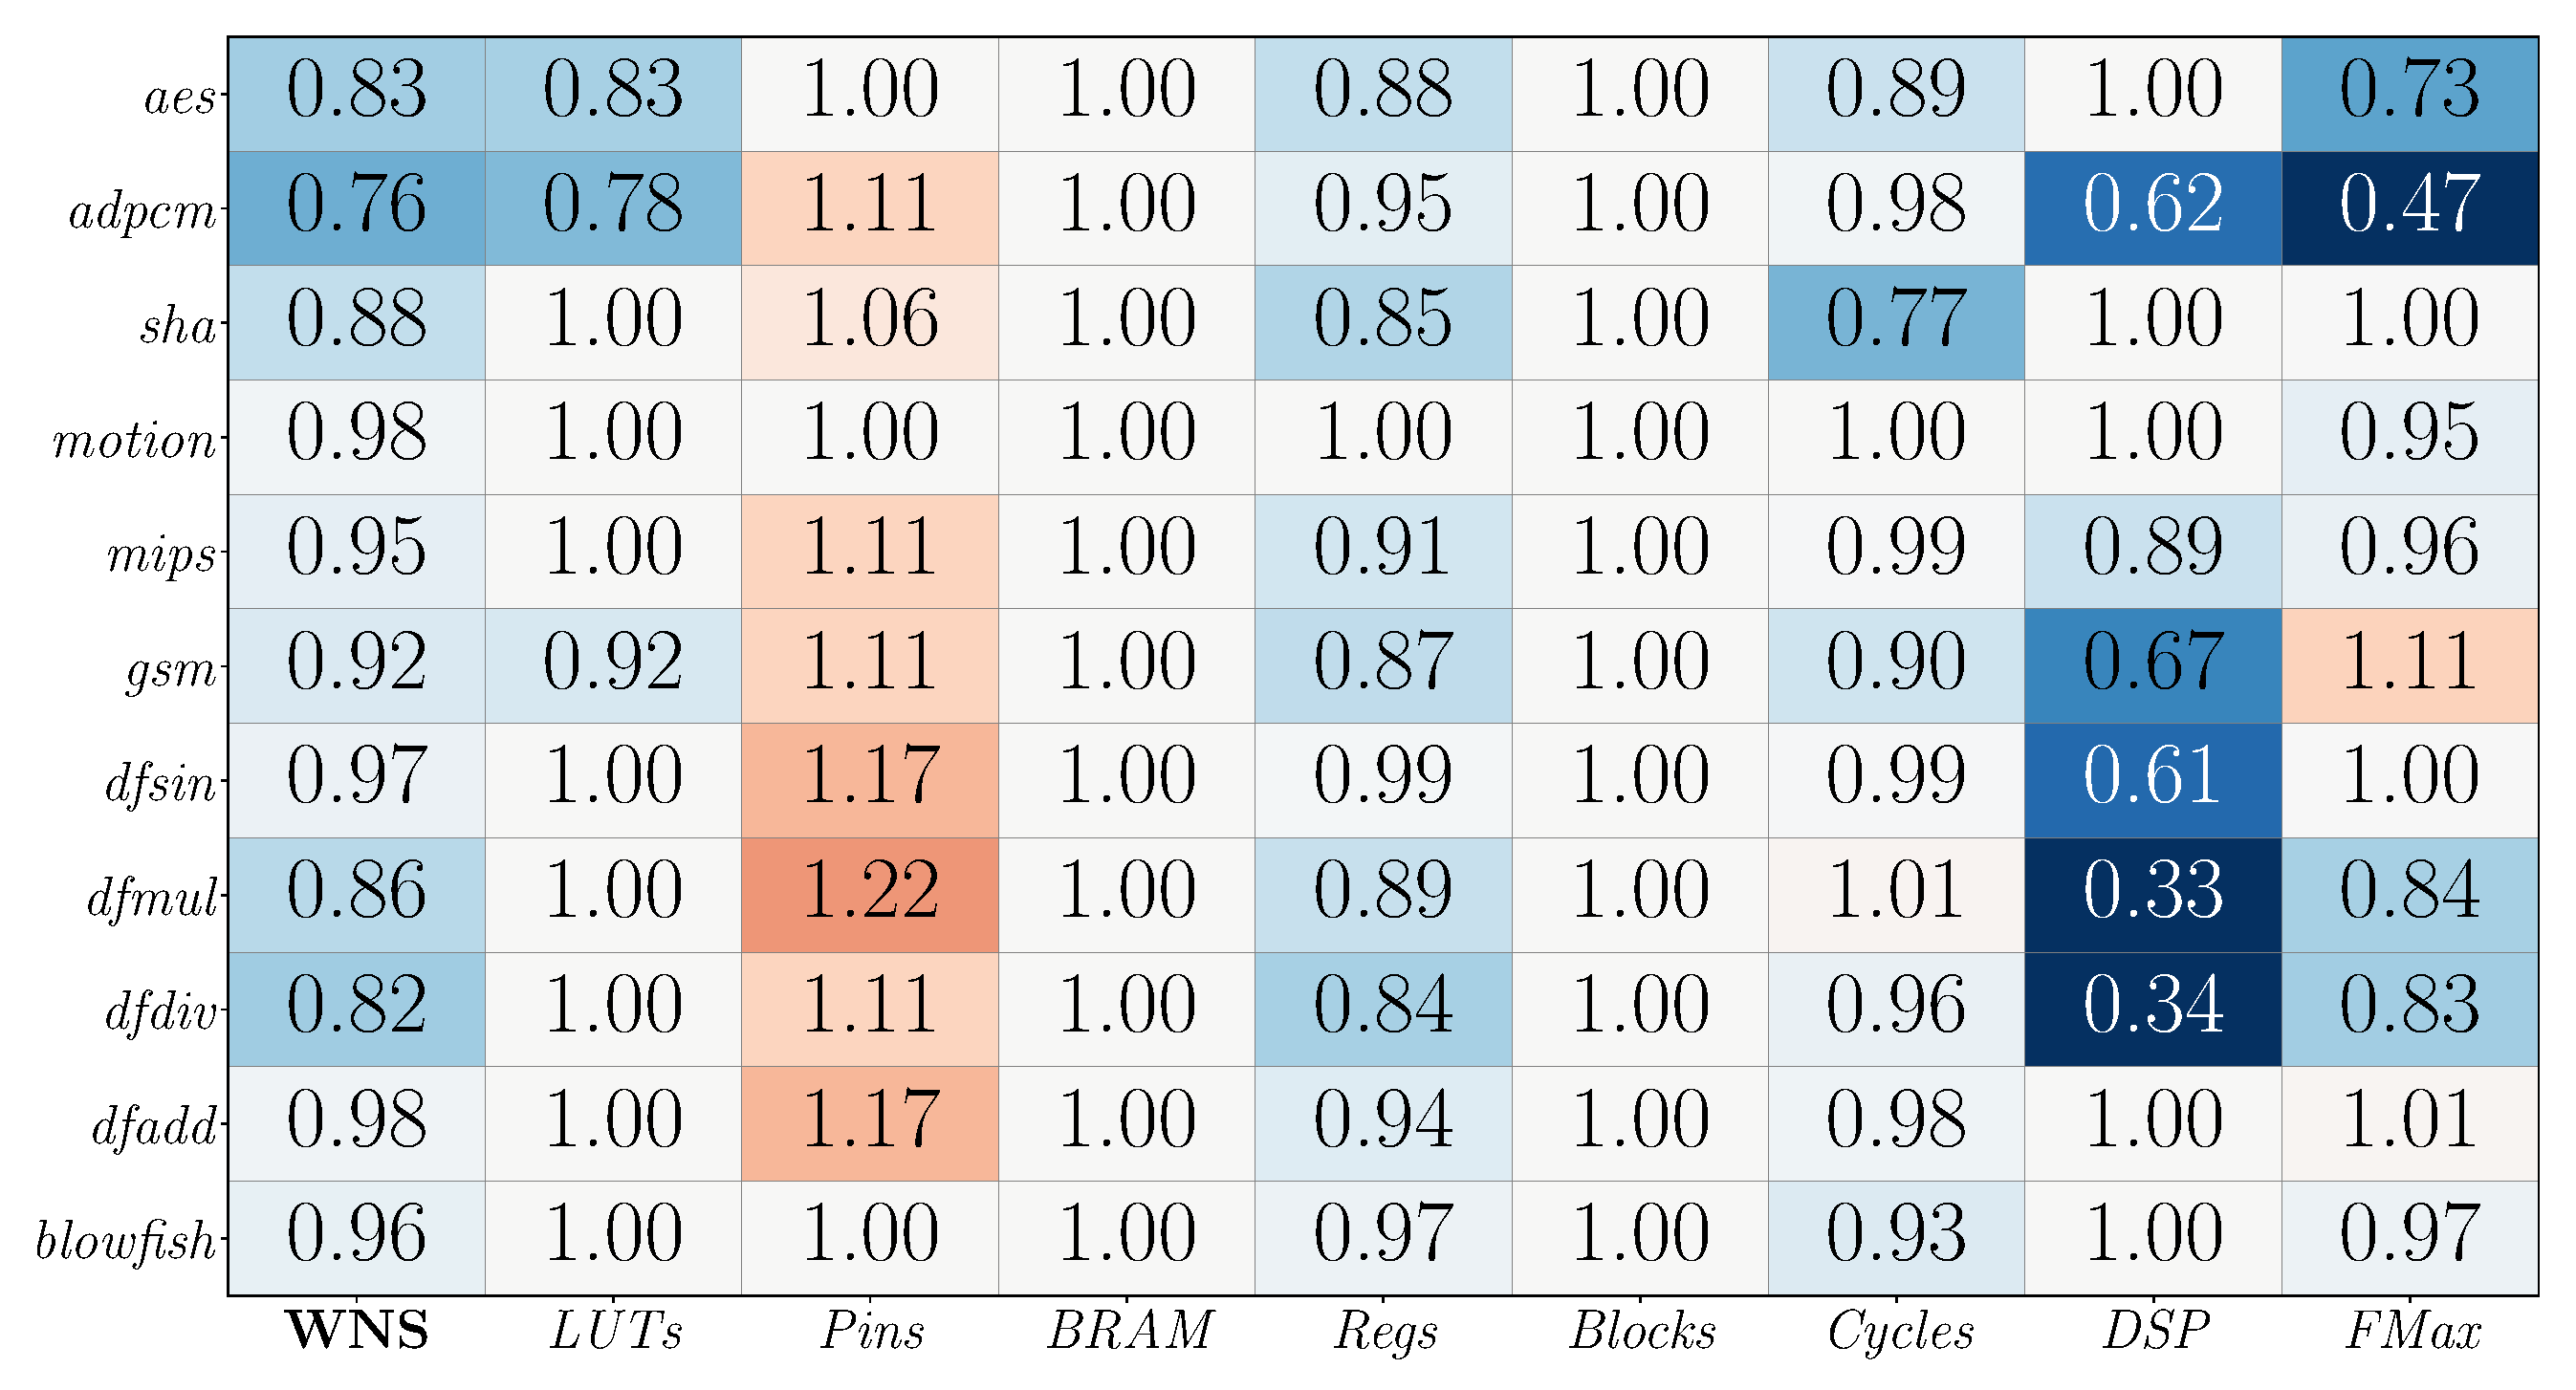
\includegraphics[width=\columnwidth]{heatmap_default_stratixV_perflat}
        \caption{Relative improvement for all metrics in the
        \textit{Performance \& Latency} scenario}
        \label{fig:perflat}
    \end{minipage}
\end{figure}

Figure \ref{fig:perflat} shows the results for the \textit{Performance \&
Latency} scenario.  The autotuner found values of \textbf{WNS} $24\%$ smaller
for \textit{adpcm}, $18\%$ smaller for \textit{dfdiv}, and smaller values
overall than in the \textit{Balanced} scenario. \textit{Regs}, \textit{Cycles}
and \textit{FMax} had higher weights in this scenario, and also better
improvements overall.  For example, $16\%$ and $15\%$ smaller \textit{Regs} in
\textit{dfdiv} and \textit{sha} respectively, $23\%$ and $11\%$ smaller
\textit{Cycles} in \textit{sha} and \textit{aes} respectively, and $53\%$
greater \textit{FMax} in \textit{adpcm}. Although \textit{FMax} had the worst
improvements in relation to the \textit{Balanced} scenario, the
\textit{Wall-Clock Time} was still decreased by the smaller values of
\textit{Cycles}.

Figure \ref{fig:wns-comp} summarizes the average improvements on \textbf{WNS}
in the 4 scenarios over 10 runs. Only the \textit{Weighted Normalized Sum} of
metrics directly guided optimization. With the exception of \textit{dfadd} in
the \textit{Balanced} scenario, the autotuner decreased \textbf{WNS} for all
applications in all scenarios by $10\%$ on average, and up to $24\%$ for
\textit{adpcm} in the \textit{Performance \& Latency} scenario. The figure also
shows the average decreases for each scenario.

\begin{figure}[htpb]
    \centering
    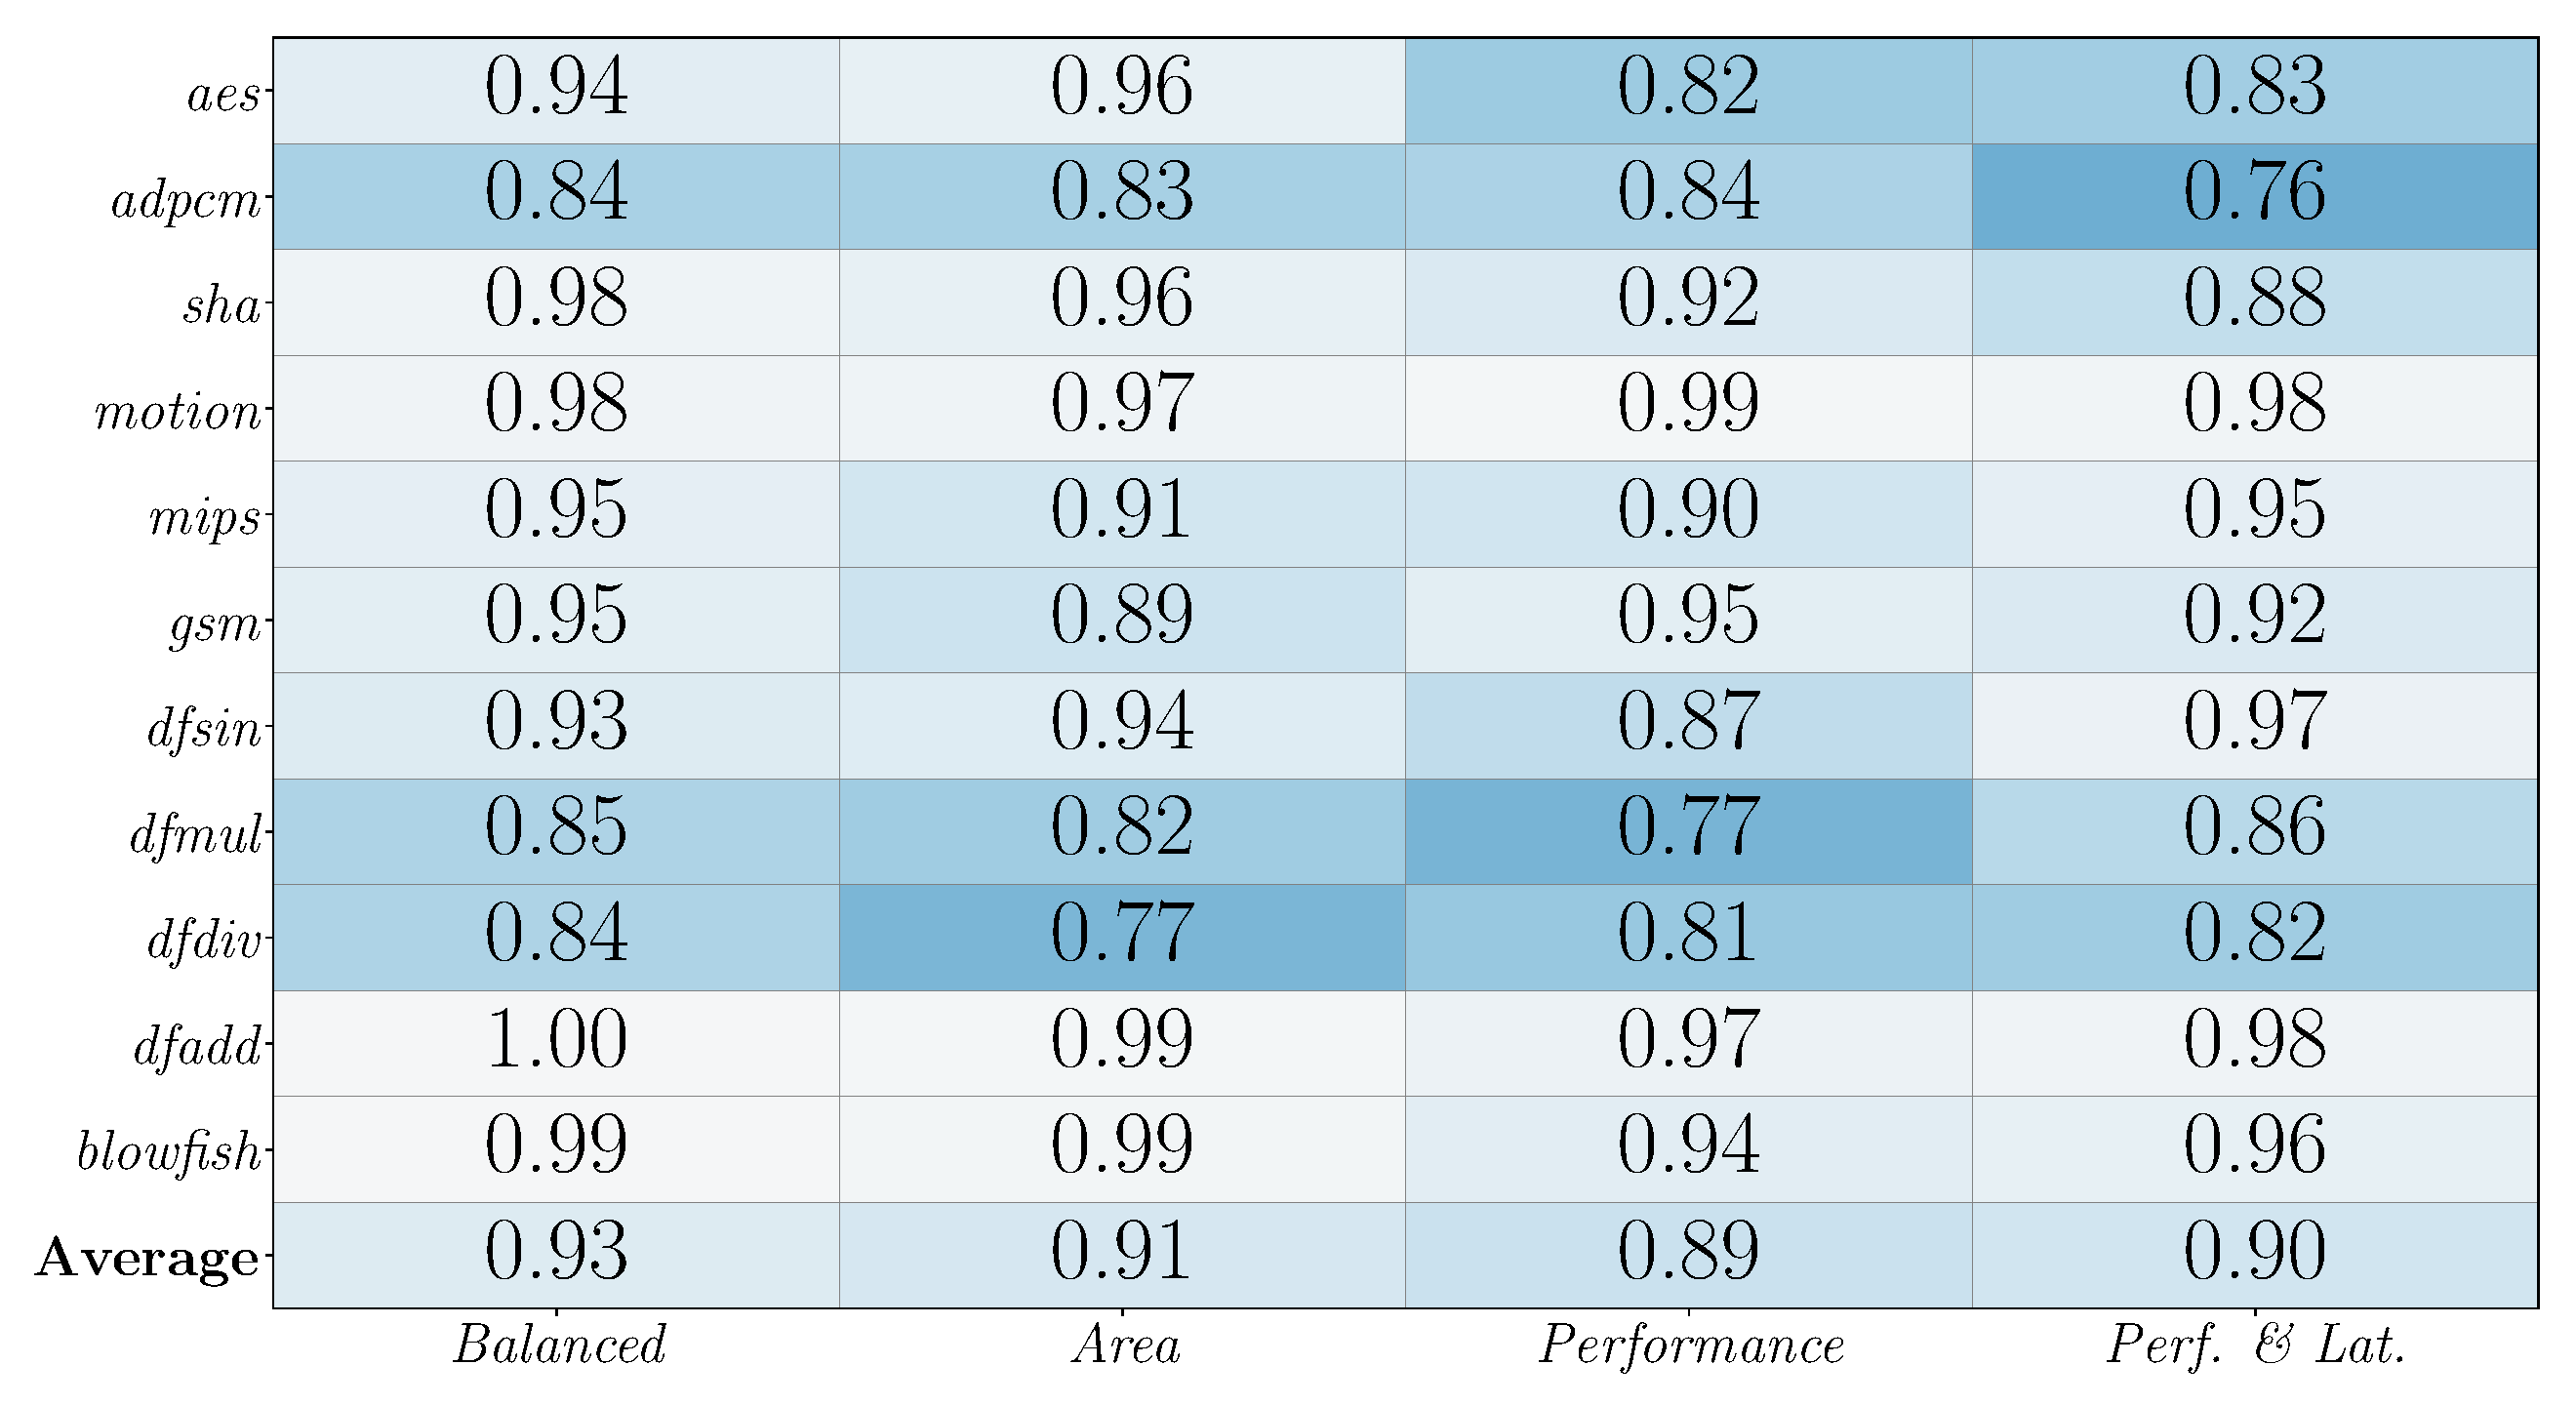
\includegraphics[width=0.5\columnwidth]{heatmap_wns_comparison}
    \caption{Relative improvement for \textbf{WNS} in all scenarios}
    \label{fig:wns-comp}
\end{figure}

\subsection{Summary}
\label{sec:FPGAconcl}

The results of this experiment show that it is always valuable to have a
sensible starting position for an autotuner. This becomes more relevant as the
size of the search space and the number of targeted metrics increase.  The
flexibility of our virtualized approach is evidenced by the results for
different optimization scenarios.  Improvements in \textbf{WNS} increased when
higher weights were assigned to metrics that express a coherent objective such
as area, performance and latency.  The improvements of metrics related to those
objectives also increased.

Future work in this direction will study the impact of different starting points on the
final tuned values in each optimization scenario, for example we could start
tuning for \textit{Performance} at the best autotuned \textit{Area} value.  We
expected that starting positions tailored for each target application will
enable the autotuner to find better \textbf{WNS} values faster.  We will also
apply this autotuning methodology to HLS tools that enable a fast prediction of
metric values. These tools will enable the exploration of the trade-off between
prediction accuracy and the time to measure an HLS configuration.
